\chapter{Results}
\label{sec:results}

% Source notes: Project/docs/thesis_notes.md (Ch. 6) and checkpoint_2026-10-10.md. Numbers:
% Project/outputs/results/<run>/{t1,t2,t3,calibration,latency,energy}/metrics.json; bootstrap: results/bootstrap/summary.md.
% Figures: Project/outputs/figures/{benchmarks,bootstrap,training-*,calibration-*}/ (copied to Thesis/images/results/).

This chapter reports the experimental results. It starts from how GroundOne learns the task and from how stable its
training is. The results on the three frozen test sets follow, together with the comparison with the baselines and the
contribution that the decision-model readout makes by itself. The chapter then examines the quality of the
probabilities, also in comparison with LLM judges that produce the same output, the time and energy needed to verify an
answer, the locality measurements (offline execution, quantisation and co-residence) and, finally, the errors that
remain. The intervals, given in parentheses in the form ``$a$ to $b$'', are 95\,\% confidence intervals obtained with a
cluster bootstrap, computed as described in Section~\ref{sec:setup-statistics}. Figure~\ref{fig:results-bootstrap}
gathers in a single plot the paired differences discussed in the chapter.

\begin{figure}[htbp]
\centering
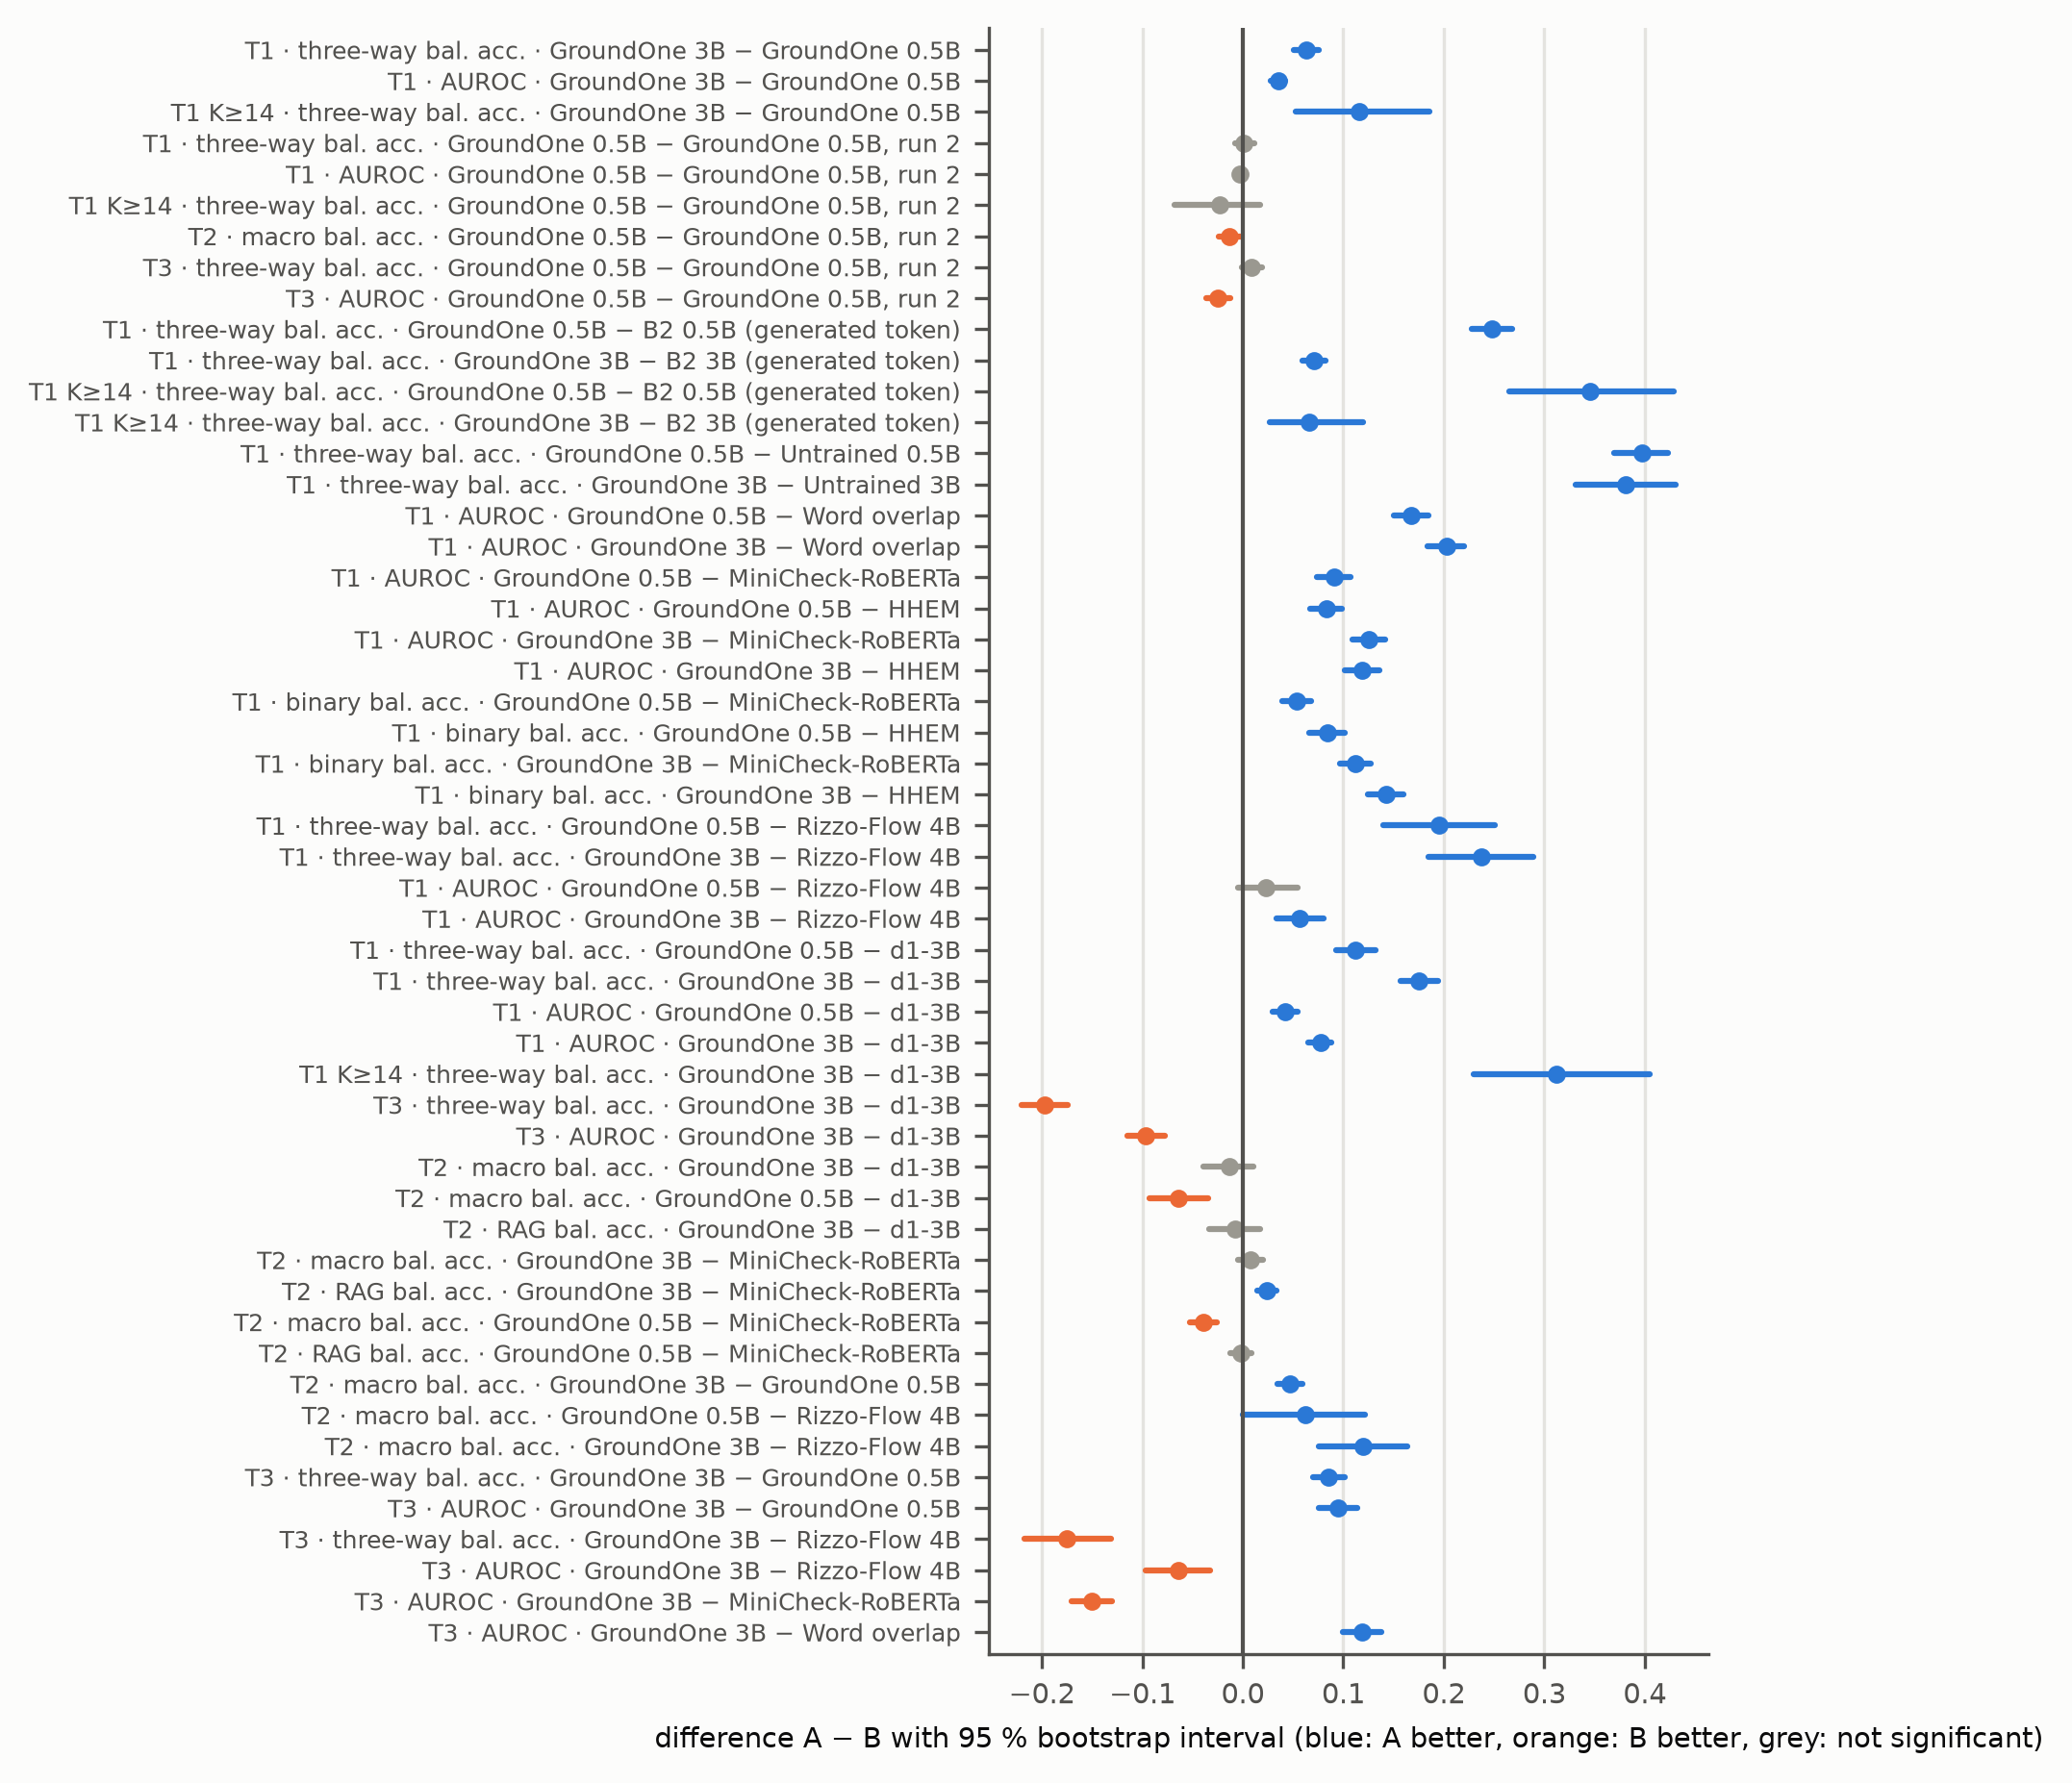
\includegraphics[width=\textwidth]{images/results/bootstrap_paired_differences.png}
\caption{All paired differences between systems on the frozen test sets, with the 95\,\% cluster-bootstrap interval. In blue the differences in favour of the first system (A), in orange those in favour of the second (B), in grey the non-significant ones, whose interval contains zero.}
\label{fig:results-bootstrap}
\end{figure}

\section{Training}
\label{sec:results-training}

Both models learned the task. Before training, a model that receives the marker format does not know what the marker
asks of it, and its verdicts are at chance: the 0.5B answers ``contradicted'' for 88\,\% of the sentences of the dev set
and reaches a three-way balanced accuracy of 0.32. In the completed runs, instead, the training loss fell within the
first hundred steps below the value of a model that knows only the class frequencies ($\ln 3 \approx 1.10$), and the
score on the dev set then rose steadily (Figure~\ref{fig:results-dev}).

The 0.5B was trained on all 13{,}203 answers and reached its best score at step 600 of 802, with a balanced accuracy
averaged over the three tasks of 0.633; from that point on the score levelled off. The 3B, trained for 12.25 hours on
6{,}500 answers, reached 0.705 at step 320 of 403, measured on its own subset of the dev set. On the whole dev set the
three-way balanced accuracy is 0.731 for the 0.5B and 0.784 for the 3B. In both runs, moreover, all three classes
remained present among the predictions throughout training.

\begin{figure}[htbp]
\centering
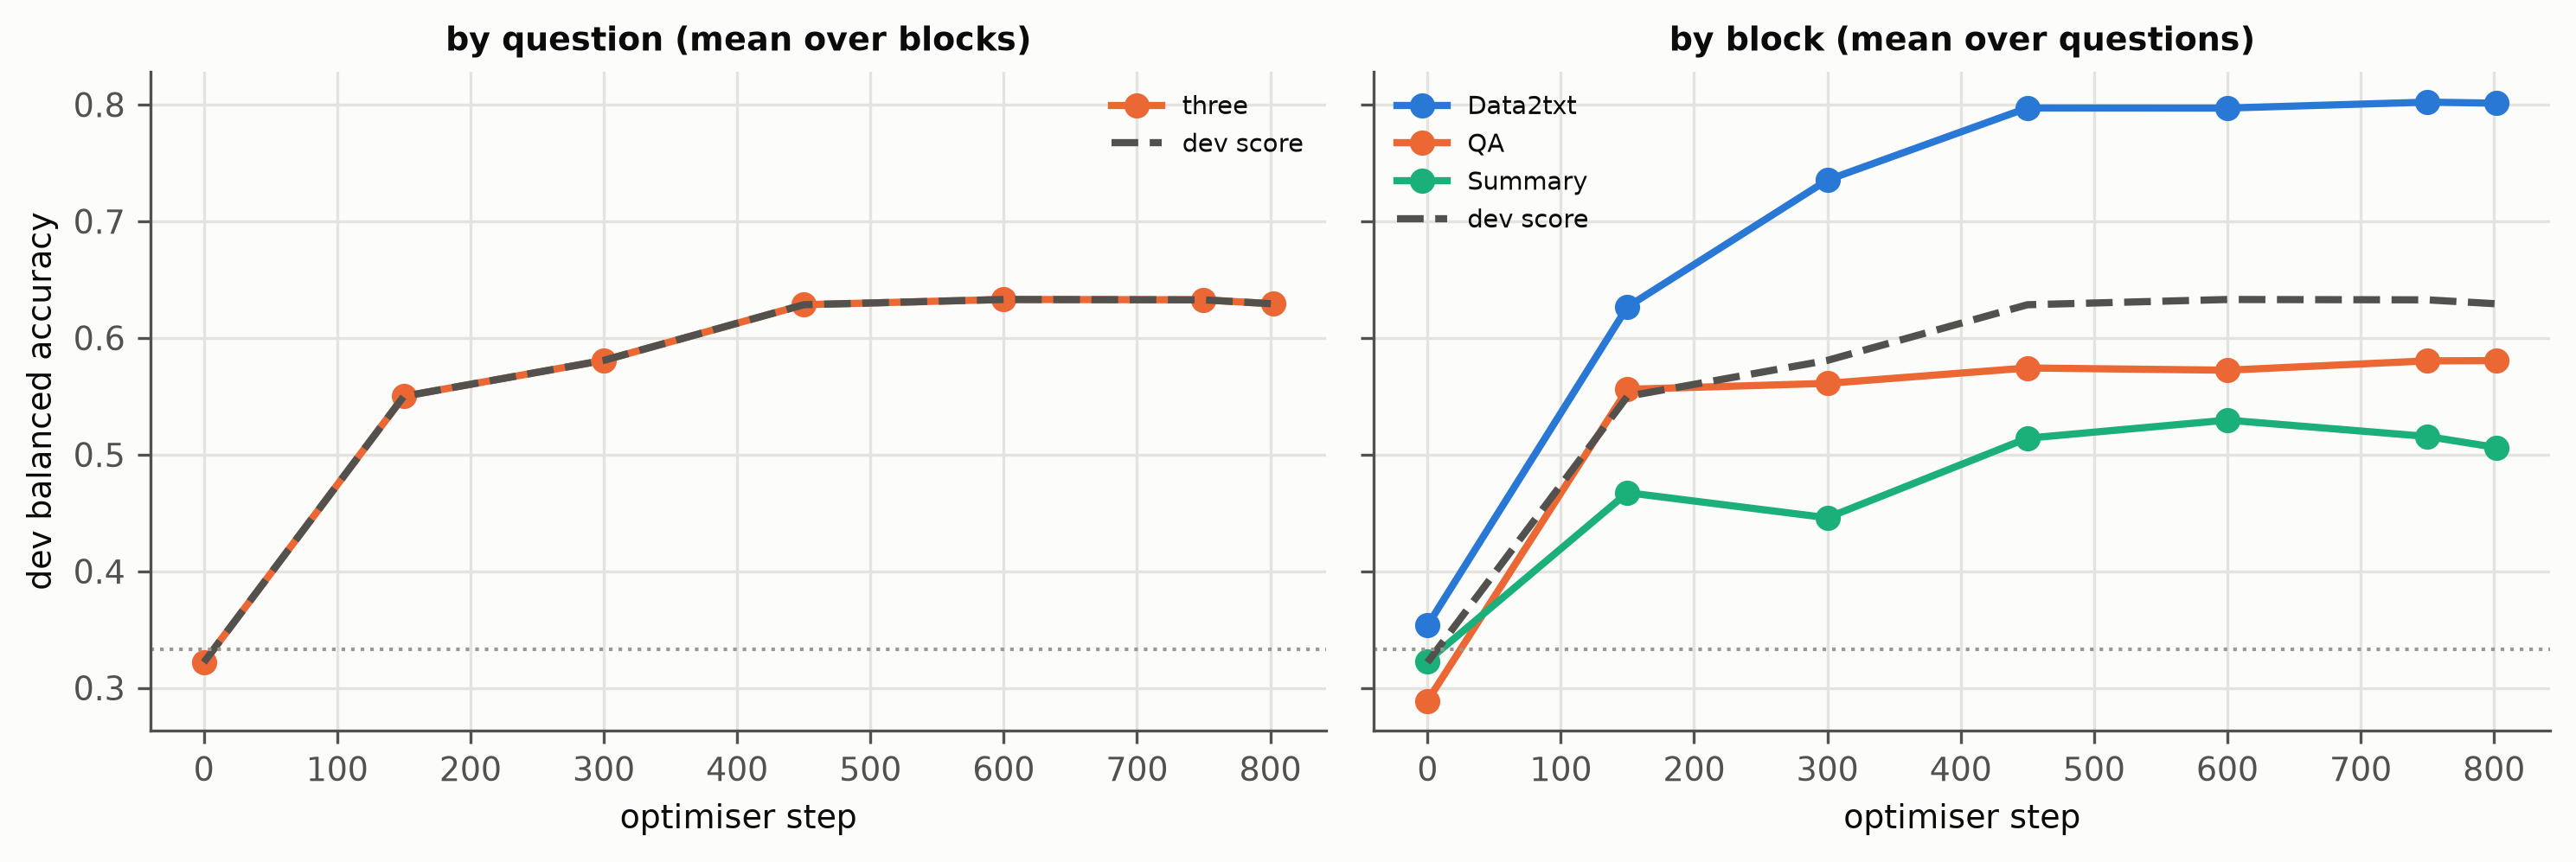
\includegraphics[width=\textwidth]{images/results/g1-05b-dev_bacc.png}
\caption{Three-way balanced accuracy on the dev set during training of the 0.5B model: overall value (left) and value
per task (right). The dotted line marks chance level. The 3B shows the same trend on its own subset of 200 answers of
the dev set.}
\label{fig:results-dev}
\end{figure}

\section{Variability across seeds}
\label{sec:results-seeds}

To understand how much the results depend on the seed, the 0.5B procedure was repeated with a second seed, which changes
the initialisation of the adapters and the order of the batches. When training converges, it converges to the same
point (Figure~\ref{fig:results-seeds}). On T1 the second run reaches a three-way balanced accuracy of 0.767, against
0.769 for the first, and an AUROC of 0.907 against 0.905. On LLM-AggreFact the macro-averaged balanced accuracy is 71.5
against 70.1, and on VitaminC the three-way balanced accuracy is 0.434 against 0.442. On T1 the paired difference
between the two runs, computed as first minus second, is $+0.001$ ($-0.008$ to $+0.012$) and is not significant.

The differences emerge in the details. First, the errors are distributed differently across the classes: the recall of
supported sentences and that of not-mentioned sentences shift by about 0.04, in opposite directions. Moreover, the
smaller slices of the data fluctuate more. The balanced accuracy of the band with fourteen or more decisions varies by
0.023, the AUROC on VitaminC by 0.025, and single datasets of LLM-AggreFact vary by up to ten points, as WiCE does (67.9
against 78.0).

\begin{figure}[htbp]
\centering
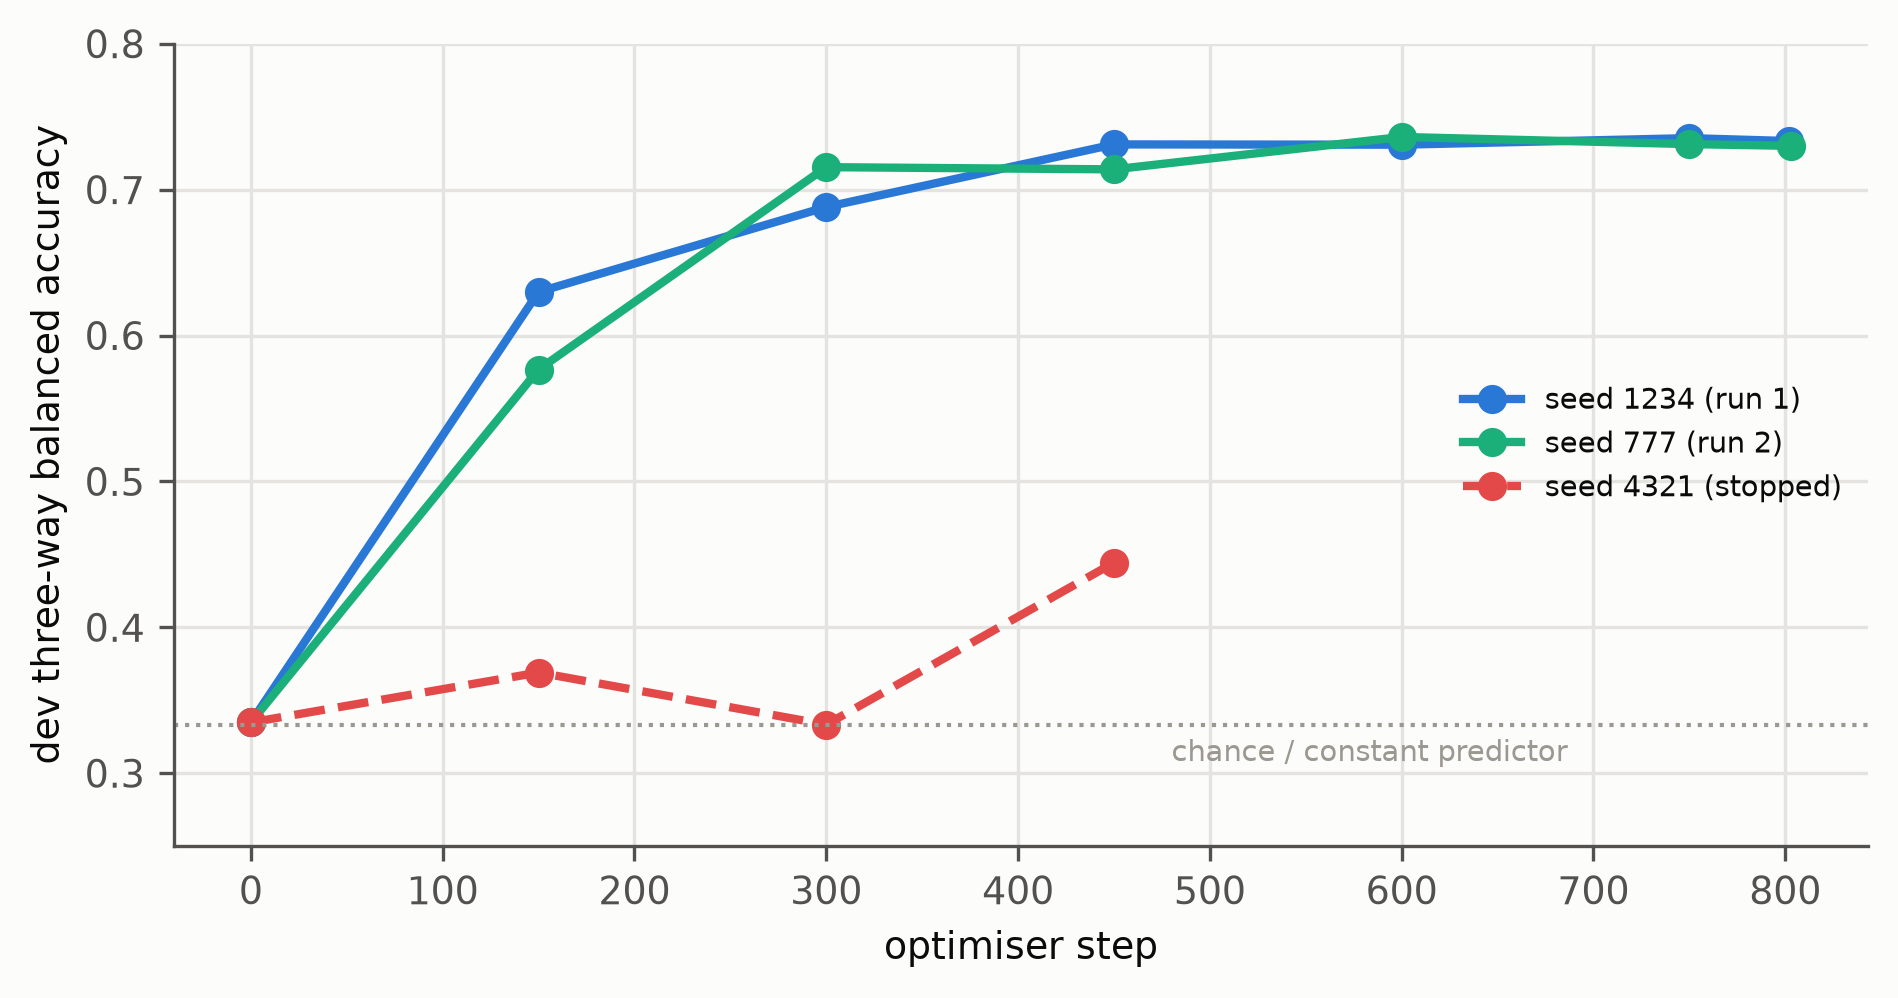
\includegraphics[width=0.85\textwidth]{images/results/seed_runs_05b.png}
\caption{Three-way balanced accuracy on the dev set during training of the 0.5B model, with the same procedure and three
different seeds. Two runs converge to the same level; the third collapsed to a constant predictor and was stopped.}
\label{fig:results-seeds}
\end{figure}

Two consequences follow from these results. The first concerns the intervals: the bootstrap resamples the test data,
and therefore does not capture the variability due to training. On LLM-AggreFact and on VitaminC, indeed, the two runs
of the same procedure differ by more than their intervals would allow (first minus second run: $-1.3$ points on the
macro average of T2, $-0.025$ on the AUROC of T3). For this reason differences between systems smaller than the spread
between seeds, that is, about 1.5 points on the macro average of LLM-AggreFact and 0.025 in AUROC on VitaminC, are not
interpreted. The same applies to single datasets of LLM-AggreFact when the gap does not exceed about five points.

The second consequence is that training does not always converge. A run with a third seed remained close to chance
level. Its score on the dev set was 0.369 at step 150 and 0.333 at step 300, when the model predicted ``supported'' for
every sentence, and the training loss remained close to that of a model without information. At step 450 the score had
climbed back to 0.444, and the run was stopped shortly afterwards, at about step 470 of 801. It is therefore not possible
to know whether it would have recovered by the end of the epoch and, being incomplete, it is excluded from the tables.
The procedure has two features that are known to make fine-tuning fragile: it applies no gradient clipping, and the
optimiser works without bias correction. The absence of bias correction is the default setting of the framework and has
been identified as one of the main causes of failed fine-tuning runs~\cite{pascanu2013difficulty,mosbach2021stability}.
A single collapse in three runs is not enough to estimate a failure rate, but it shows that the procedure is not fully
robust to initialisation.

\section{Accuracy on the RAG test set (T1)}
\label{sec:results-t1}

On the 17{,}284 sentences of T1 the 0.5B model reaches a three-way balanced accuracy of 0.769 and the 3B of 0.832
(Table~\ref{tab:results-t1}). The difference between the two, $+0.063$ ($+0.051$ to $+0.076$), is the clearest effect of
model size. On the binary decision the 0.5B obtains a balanced accuracy of 0.815 and an AUROC of 0.905, while the 3B
obtains 0.874 and 0.940 respectively. Both are far above the cues that never compare a sentence with its document: word
overlap reaches an AUROC of 0.737, and the classifier that sees only the sentence reaches a three-way balanced accuracy
of 0.570.

\begin{table}[htbp]
\centering
\caption{GroundOne on T1, on the whole test set, by task and by number of decisions per answer ($K$). For each model the
three-way balanced accuracy, the recall of contradicted sentences and the AUROC of $P(\text{supported})$ are reported.
$^{*}$Indicative value: the cell contains fewer than 30 contradicted sentences.}
\label{tab:results-t1}
\small
\begin{adjustbox}{max width=\textwidth}
\begin{tabular}{@{}lrrrrrrr@{}}
\toprule
 & & \multicolumn{3}{c}{GroundOne 0.5B} & \multicolumn{3}{c}{GroundOne 3B} \\
\cmidrule(lr){3-5}\cmidrule(l){6-8}
Subset & Sentences & Bal.\ acc. & Contr. & AUROC & Bal.\ acc. & Contr. & AUROC \\
\midrule
All & 17{,}284 & 0.769 & 0.68 & 0.905 & 0.832 & 0.76 & 0.940 \\
\midrule
Question answering & 4{,}876 & 0.589 & 0.03$^{*}$ & 0.916 & 0.699 & 0.30$^{*}$ & 0.948 \\
Summarisation & 4{,}538 & 0.544 & 0.13 & 0.775 & 0.629 & 0.30 & 0.873 \\
Data-to-text & 7{,}870 & 0.812 & 0.84 & 0.929 & 0.873 & 0.90 & 0.955 \\
\midrule
$K$ = 1--4 & 2{,}434 & 0.606 & 0.18 & 0.857 & 0.677 & 0.25 & 0.921 \\
$K$ = 5--8 & 8{,}012 & 0.758 & 0.67 & 0.899 & 0.829 & 0.78 & 0.936 \\
$K$ = 9--13 & 5{,}201 & 0.824 & 0.82 & 0.926 & 0.863 & 0.86 & 0.945 \\
$K \geq 14$ & 1{,}637 & 0.723 & 0.50 & 0.908 & 0.839 & 0.68 & 0.957 \\
\bottomrule
\end{tabular}
\end{adjustbox}
\end{table}

Three aspects emerge from the table. The first is that accuracy does not collapse with the length of the answer. Answers
with fourteen or more decisions reach a balanced accuracy of 0.839 with the 3B, among the best, and of 0.723 with the
0.5B, slightly below the intermediate bands. The hardest band is instead that of the shortest answers, which mostly
contains question-answering and summarisation answers. The finding matters because it is precisely on long answers that
a decision model saves the most time; on these answers the 3B gains $+0.116$ ($+0.053$ to $+0.186$) over the 0.5B.

The second aspect is that contradictions are recognised mainly in data-to-text, the task in which RAGTruth concentrates
them. In question answering and summarisation the 0.5B separates supported from not-mentioned sentences well, but finds
almost no contradictions: the recall of contradicted sentences is 0.03 and 0.13, and the first value is only
indicative, because in question answering there are fewer than 30 contradicted sentences. The 3B raises it to 0.30 in
both tasks, so model size compensates in part for the scarcity of these examples in the training data. The third aspect
is that question answering and summarisation offer the clearest evidence that the models really read the document. In
these two tasks the classifier that sees only the sentence stays at chance level (0.36 and 0.35), while the two models
reach 0.59--0.70 in question answering and 0.54--0.63 in summarisation.

The same predictions can also be evaluated at the level of the whole answer. This is the criterion with which the
community Decision Index evaluates general-purpose decision models on RAGTruth: an answer is hallucinated if it contains
any unsupported content, and the metric is the F1 score of this class. A system that always answers ``hallucinated''
already reaches an F1 of 0.52~\cite{decisionindex2026}. To judge an answer, GroundOne takes the minimum of the
calibrated $P(\text{supported})$ over its sentences and compares it with a threshold fitted on the dev set. With this
rule, on the 2{,}647 answers of T1 it reaches an F1 of 0.733 with the 0.5B and of 0.784 with the 3B. On the leaderboard,
by contrast, no general-purpose decision model below one billion parameters exceeds 0.553, Jev reaches 0.765 and the
best model, of 27B parameters, 0.803. The comparison is only indicative, because GroundOne was trained on RAGTruth,
whereas the leaderboard models are evaluated zero-shot, with a different prompt and on 53 more answers. It nevertheless
places a 0.5B specialist far above the general-purpose decision models of the same size.

\section{Comparison with the baselines}
\label{sec:results-baselines}

Figure~\ref{fig:results-comparison} compares all systems on T1. The specialised encoders reach an AUROC of 0.814
(MiniCheck-RoBERTa) and 0.821 (HHEM): more than word overlap, but less than both GroundOne models. The 0.5B exceeds
MiniCheck-RoBERTa by $+0.091$ ($+0.074$ to $+0.108$) and HHEM by $+0.083$ ($+0.067$ to $+0.099$); the 3B exceeds them by
$+0.126$ and $+0.119$ respectively. The comparison by task, however, qualifies this result. GroundOne's advantage comes
largely from data-to-text, where it benefits from in-domain training and from the recurring structure of the templates,
and where the encoders are weakest (AUROC 0.71--0.75). In summarisation, instead, MiniCheck-RoBERTa outperforms the 0.5B
model (0.872 against 0.775) and is on par with the 3B (0.873). Figure~\ref{fig:results-by-task} reports the AUROC per
task of all systems.

\begin{figure}[htbp]
\centering
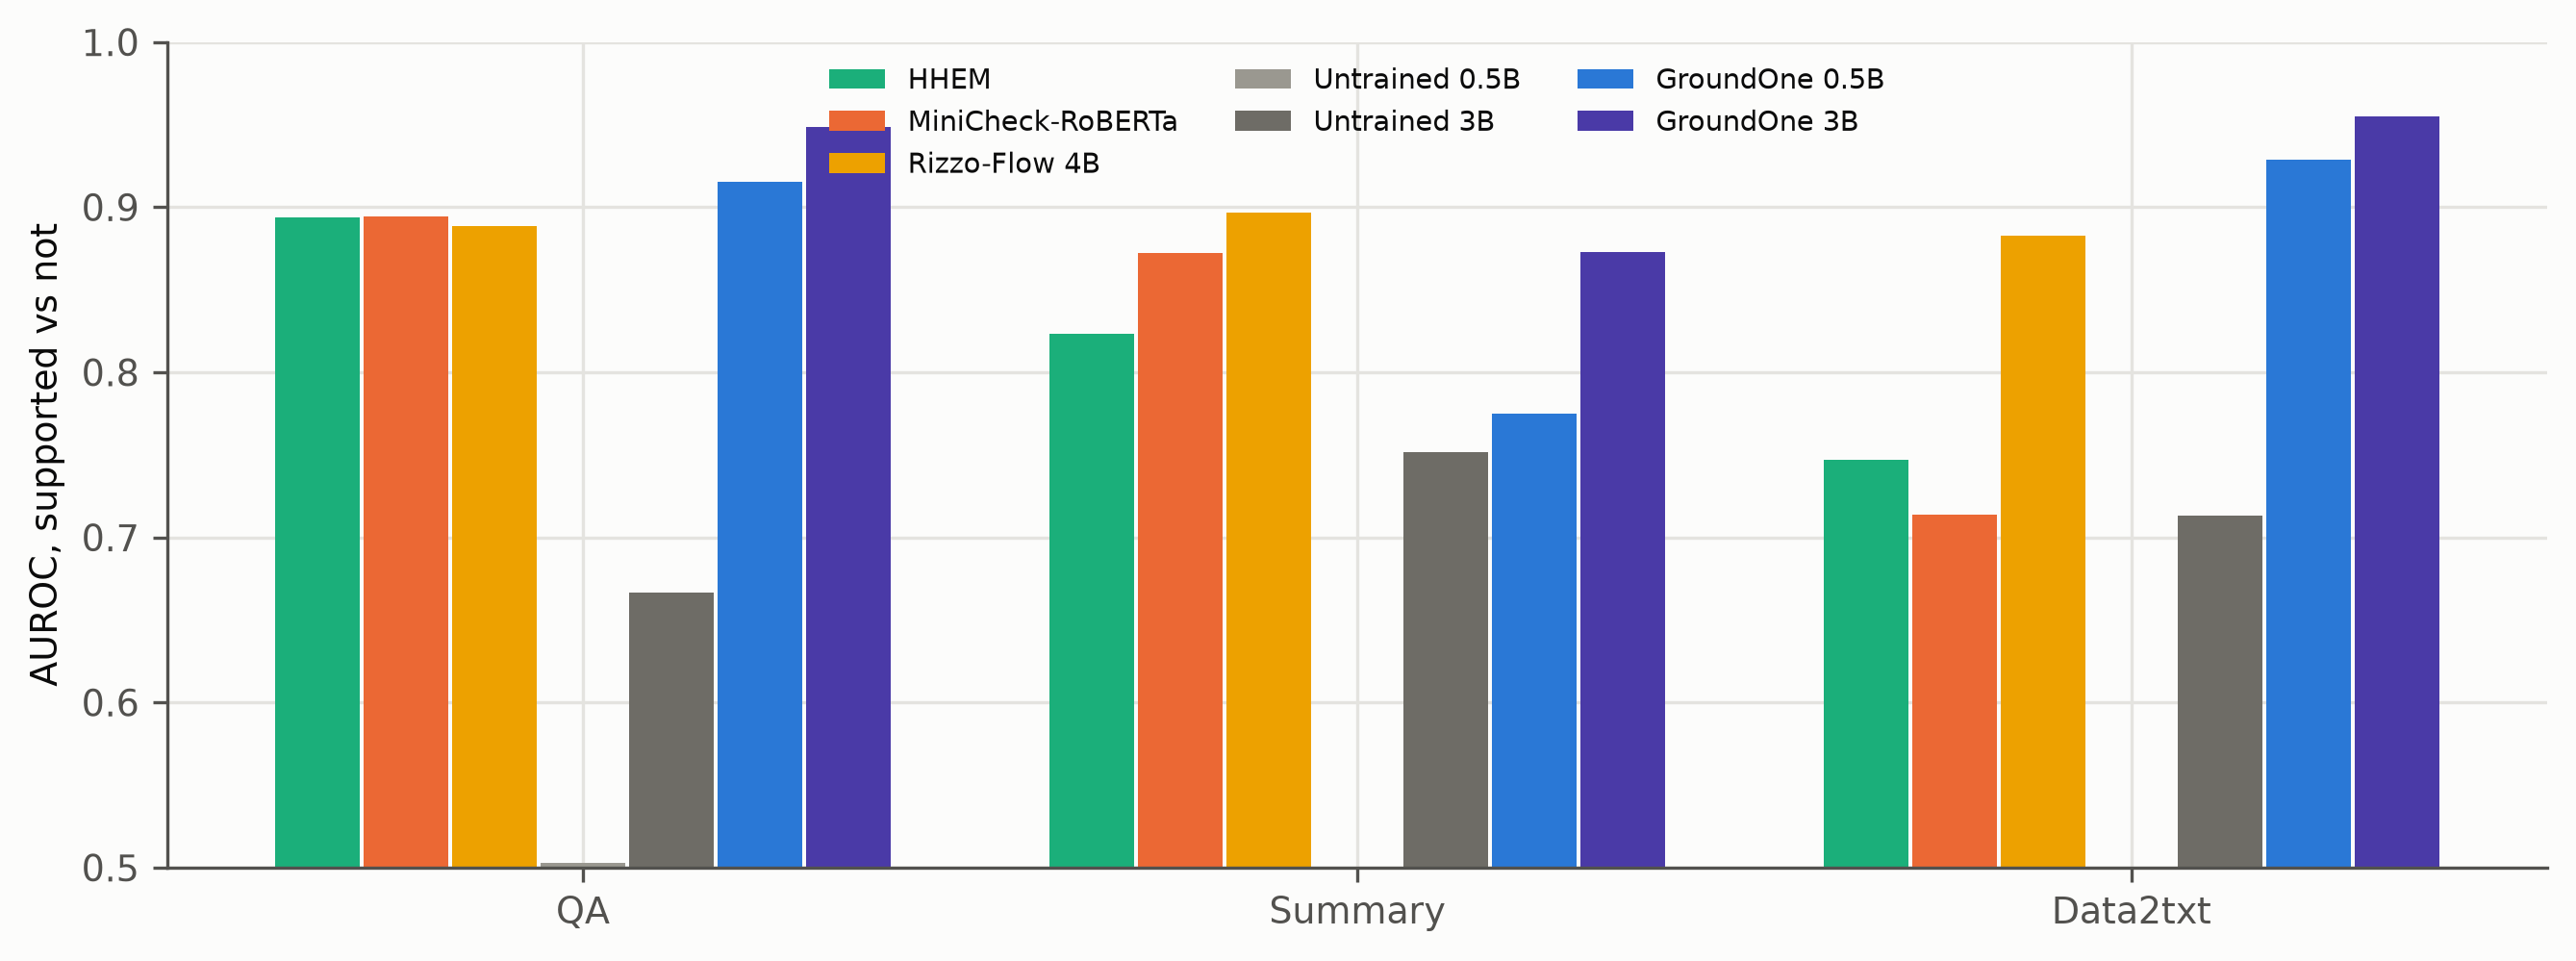
\includegraphics[width=\textwidth]{images/results/t1_by_task.png}
\caption{AUROC of $P(\text{supported})$ on T1 by task (question answering, summarisation, data-to-text) and by system. GroundOne's advantage is concentrated in data-to-text; in summarisation MiniCheck-RoBERTa outperforms the 0.5B and is on par with the 3B.}
\label{fig:results-by-task}
\end{figure}

The untrained models show how much of the accuracy is due to training. The untrained 0.5B is at chance level, with a
three-way balanced accuracy of 0.372, because it never answers ``supported''. The untrained 3B, asked the same question,
reaches a three-way balanced accuracy of 0.437, against 0.818 for the same model after training, on the same answers.
The contribution of the restricted readout, beyond training, is measured separately in Section~\ref{sec:results-readout}.

\begin{figure}[htbp]
\centering
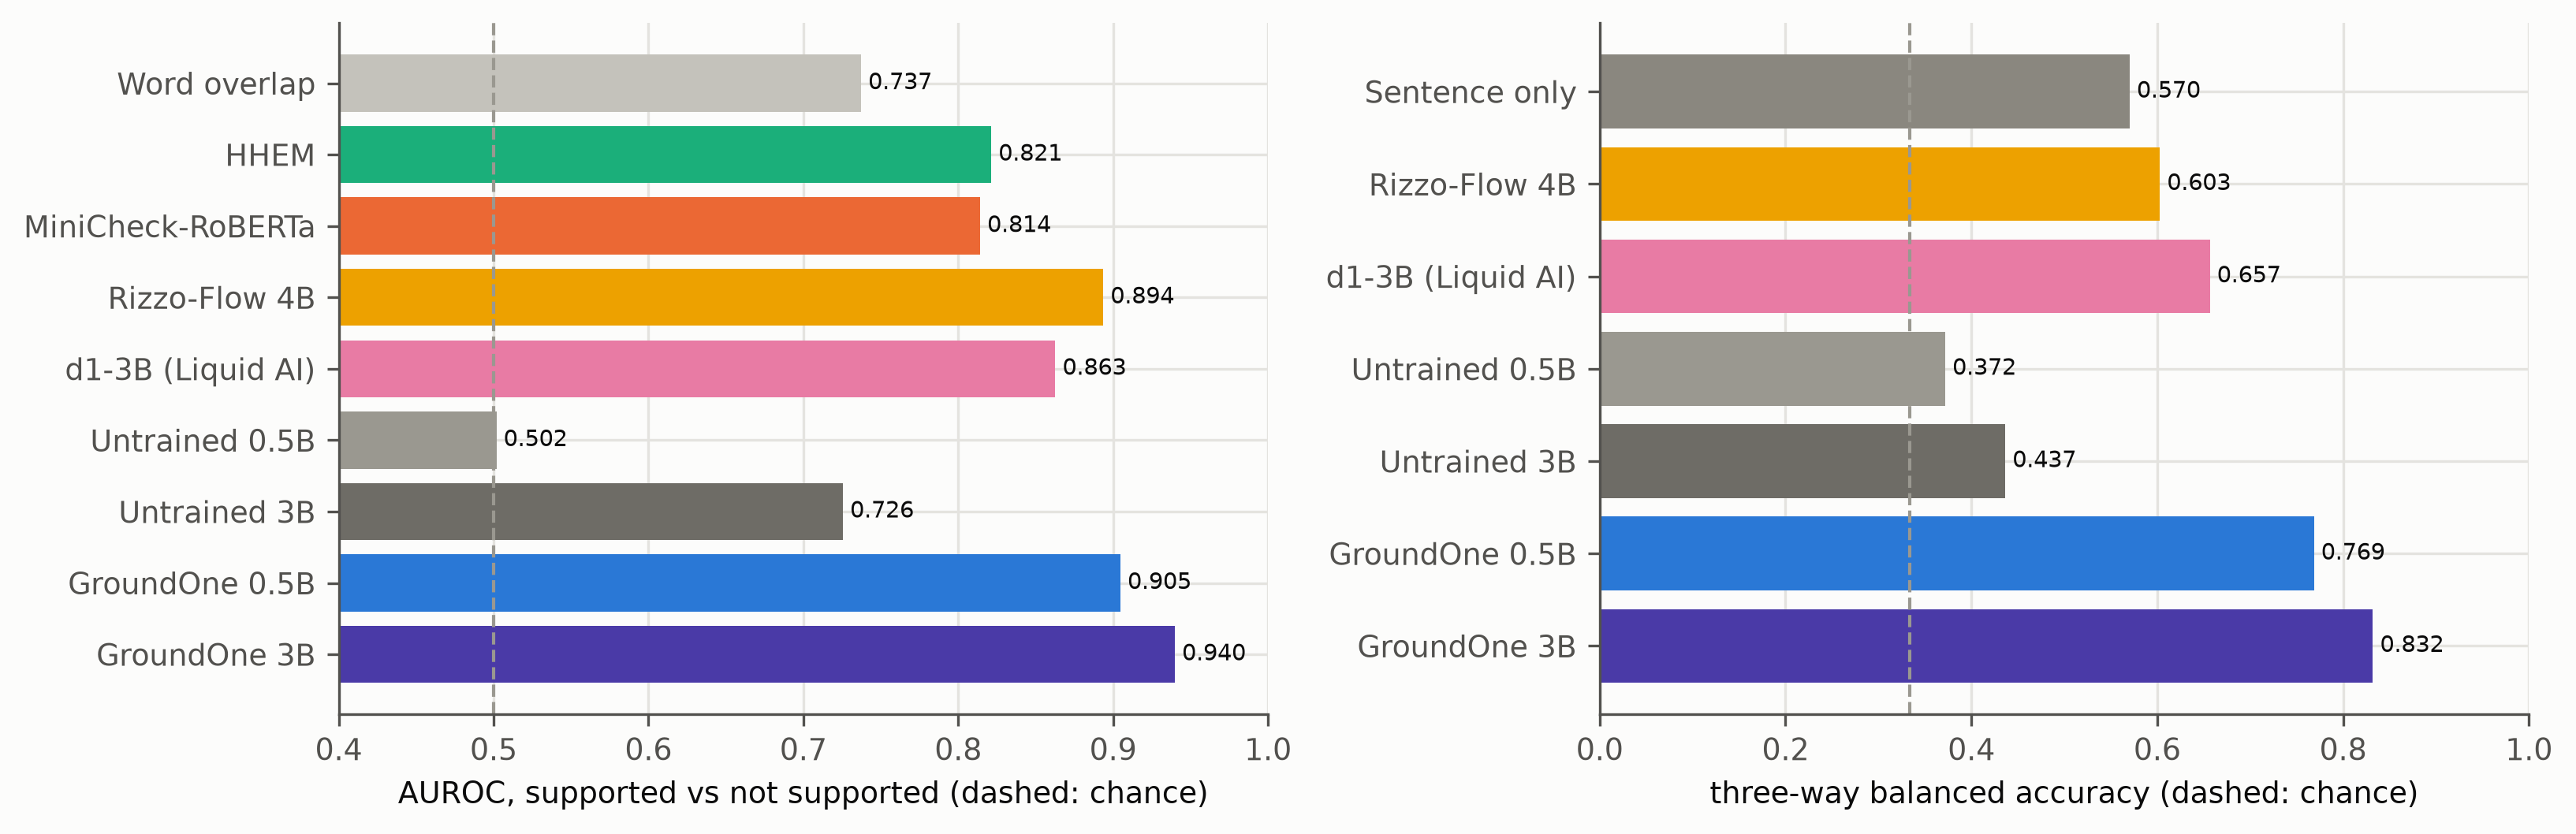
\includegraphics[width=\textwidth]{images/results/comparison_t1.png}
\caption{T1: AUROC of $P(\text{supported})$ for every system (left) and three-way balanced accuracy for the systems with
a three-way output (right). Rizzo-Flow is evaluated on 300 answers and the untrained 3B on 600; all other systems,
including d1-3B, are evaluated on the whole test set.}
\label{fig:results-comparison}
\end{figure}

The most instructive comparison is the one with Rizzo-Flow, the larger general-purpose decision model: a 4B model
fine-tuned for generic decisions. On the same 300 answers of T1, Rizzo-Flow reaches a three-way balanced accuracy of
0.603, against 0.798 for the 0.5B GroundOne and 0.840 for the 3B. The differences are large: $+0.195$ ($+0.140$ to
$+0.251$) for the 0.5B and $+0.237$ ($+0.184$ to $+0.289$) for the 3B. In AUROC, by contrast, Rizzo-Flow (0.894) is
close to the 0.5B, which obtains 0.916 on these answers, and the difference is not significant. Rizzo-Flow, in fact,
ranks the sentences well, but predicts ``supported'' for 90\,\% of them. The 3B ranks them better than Rizzo-Flow
($+0.056$, $+0.034$ to $+0.081$). A specialist eight times smaller therefore outperforms the generalist on the decision
it was designed for and matches it in the ability to rank sentences.

d1-3B, a general-purpose decision model of the same size as the 3B, offers the strictest test of the value of
specialisation. It is in fact already trained to make typed decisions, and it differs from GroundOne mainly in the data
on which it was trained. On the whole of T1 it reaches a three-way balanced accuracy of 0.657 and an AUROC of 0.863.
Both GroundOne models do clearly better. The 0.5B, six times smaller, exceeds it by $+0.112$ ($+0.092$ to $+0.133$) in
three-way balanced accuracy and by $+0.042$ in AUROC; the 3B exceeds it by $+0.175$ ($+0.157$ to $+0.195$) and by
$+0.077$. The gap is widest on long answers: when the answer contains fourteen or more decisions, d1-3B drops to 0.527,
while the 3B GroundOne stays at 0.839 ($+0.312$, $+0.230$ to $+0.405$). Moreover, d1-3B recognises only half of the
not-mentioned sentences (recall 0.49). Within the domain of RAG answers, then, specialisation is worth far more than a
generic training to make decisions.

On LLM-AggreFact (T2) the 0.5B model reaches a macro-averaged balanced accuracy of 70.1 over the eleven datasets,
against 64.2 for the same model used zero-shot (the score published on the leaderboard) and 72.8 for the zero-shot 7B
model reported on the public leaderboard. It remains, however, 3.9 points below MiniCheck-RoBERTa (74.0), a significant
difference. On the four datasets closest to retrieval-augmented generation the two systems are on par (74.4 for
GroundOne 0.5B, 74.6 for MiniCheck-RoBERTa). On the RAGTruth column GroundOne leads, 82.1 against 76.5, but the
comparison favours it, because it was trained on the answers of the RAGTruth training set. Outside RAG, instead, the
0.5B is seven to nine points below the encoder on AggreFact-CNN, AggreFact-XSum, FactCheck-GPT and REVEAL: this is the
expected cost of training on RAG data alone.

The 3B model, evaluated on the whole test set, closes most of this gap. Its macro-averaged balanced accuracy is 74.8: it
is on par with that of MiniCheck-RoBERTa (74.0; paired difference $+0.8$ points, interval $-0.5$ to $+2.0$) and above
the published zero-shot score of the 7B model (72.8), for which no interval can be computed. On the RAG datasets it
reaches 76.9, 2.4 points above the encoder (interval $+1.4$ to $+3.4$). Its gain over the 0.5B, $+4.7$ points ($+3.4$
to $+5.9$), is spread across the datasets, with the largest improvements on REVEAL, WiCE, FactCheck-GPT and XSum: model
size therefore improves transfer beyond the training domain. The 3B remains clearly below the encoder only on news
summarisation (AggreFact-CNN, 59.3 against 67.1). Rizzo-Flow reaches 61.5 on the 1{,}093 items of its subsample, and on
these items the 3B GroundOne does better by 12.0 points ($+7.6$ to $+16.4$).

On this benchmark, however, the strongest systems remain above GroundOne. An independent evaluation of the closed
decision model Jev, on the same test set and with the same metric, reports 78.6, and 76.9 for a 27B open model read
through its answer letters. The prompts differ from those used here, and no interval can be
computed~\cite{deusser2026jev}. On a broad groundedness benchmark, then, a 3B specialist trained only on RAG answers
matches the best small encoder, but remains below the closed state of the art and below much larger open models. The
general-purpose d1-3B confirms the picture when the size is the same. On a random subsample of 4{,}000 items it reaches
75.7, against 74.3 for the 3B GroundOne on the same items, a difference that is not significant ($-1.3$, $-4.0$ to
$+1.0$), while it exceeds the 0.5B by 6.5 points. Compared with the 3B GroundOne, d1-3B is weaker on the RAGTruth column
(78.9 against 87.3) and clearly stronger on WiCE and on dialogue summarisation.

\section{Transfer to a different domain (T3)}
\label{sec:results-t3}

On VitaminC the picture reverses. On the whole test set the 0.5B reaches a three-way balanced accuracy of 0.442 and the
3B of 0.527, with an AUROC of 0.722 and 0.817 respectively, while MiniCheck-RoBERTa reaches an AUROC of 0.968. On the
600 pairs evaluated with Rizzo-Flow, the general-purpose model obtains a three-way balanced accuracy of 0.712 and an
AUROC of 0.909, against 0.442 and 0.744 for the 0.5B and 0.537 and 0.845 for the 3B.
Figure~\ref{fig:results-comparison-t3} shows the complete comparison on T3.

\begin{figure}[htbp]
\centering
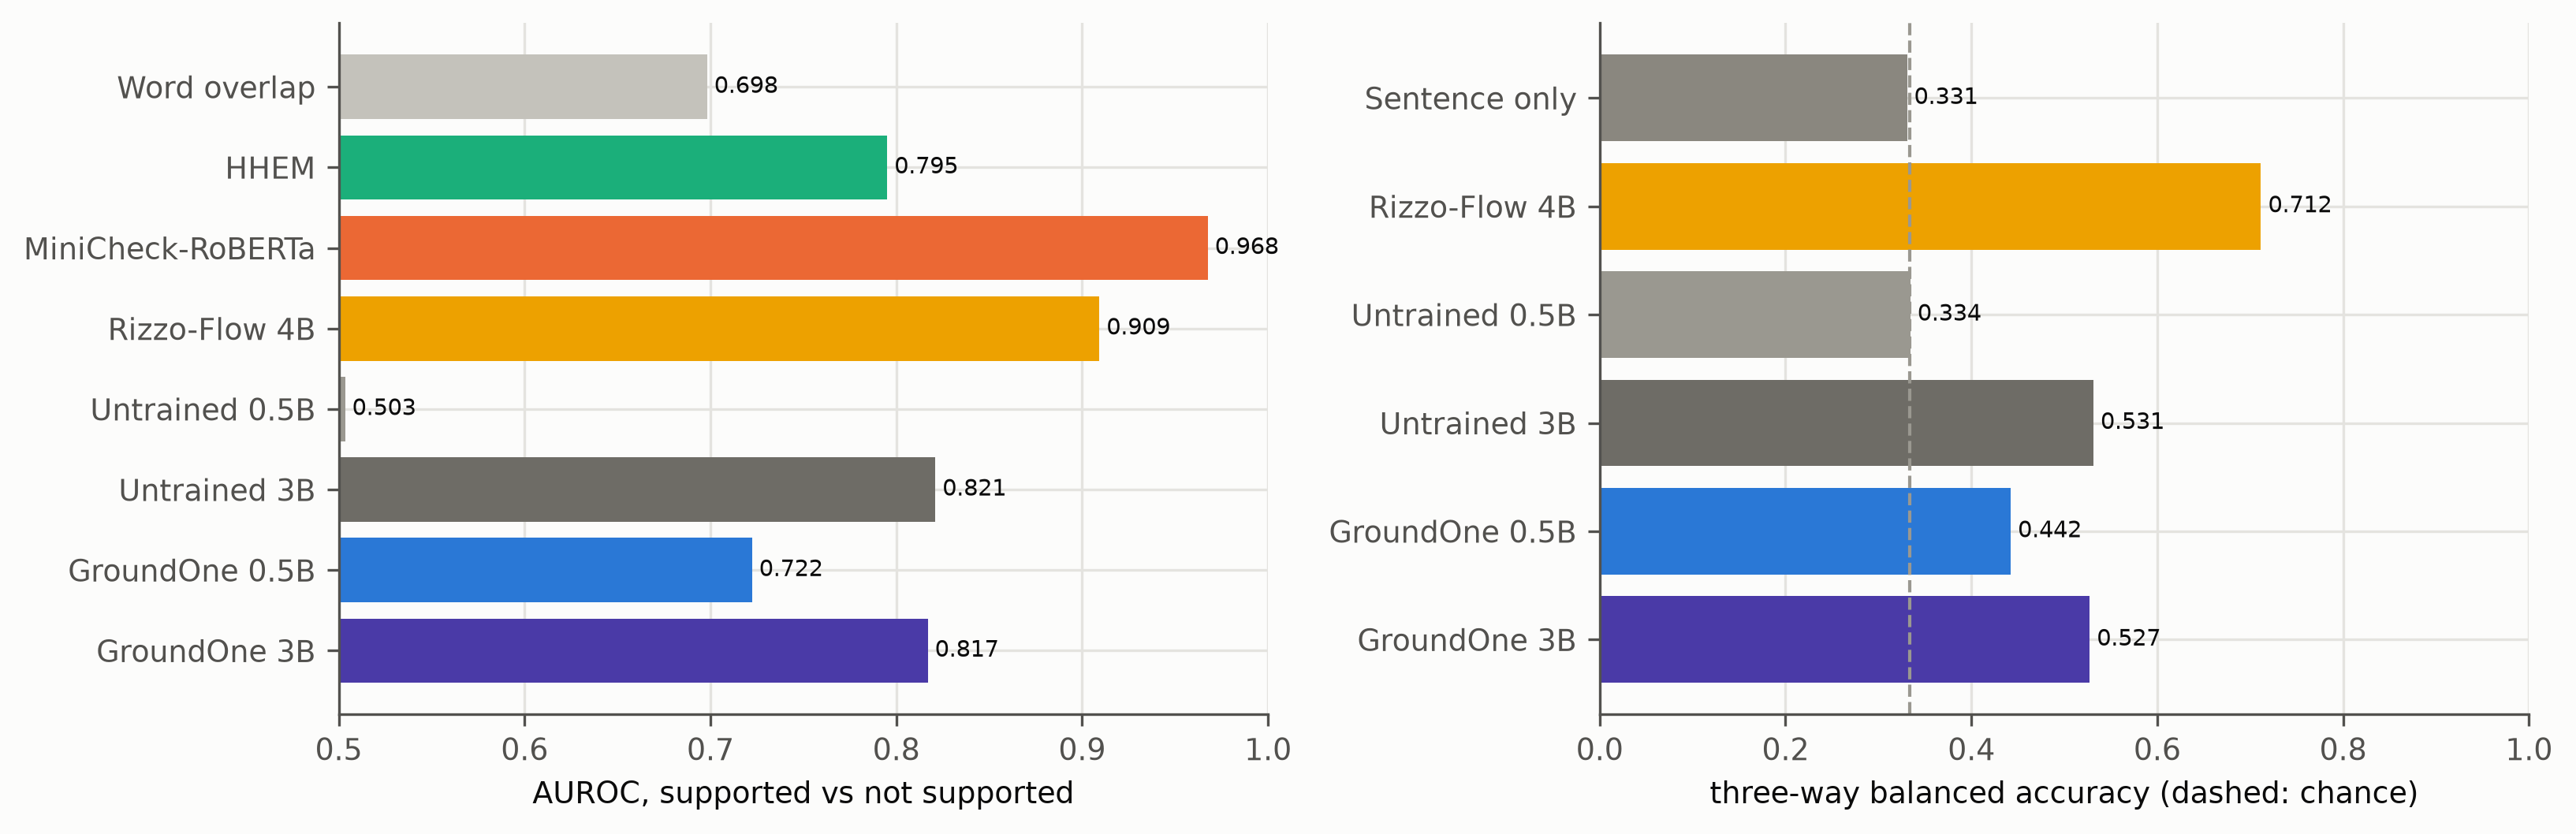
\includegraphics[width=\textwidth]{images/results/comparison_t3.png}
\caption{Comparison of the systems on T3 (VitaminC): on the left the AUROC of $P(\text{supported})$, on the right the three-way balanced accuracy for the systems with a three-way output. Rizzo-Flow is evaluated on a subsample of 600 pairs; the dashed line marks chance level. For MiniCheck-RoBERTa, VitaminC is part of the lineage of its training data.}
\label{fig:results-comparison-t3}
\end{figure}

Two facts help to interpret these numbers. The first is that MiniCheck-RoBERTa starts from the AlignScore model, whose
training data include VitaminC~\cite{zha2023alignscore}. For the encoder, therefore, T3 belongs to the training
distribution, whereas for GroundOne it measures transfer from RAGTruth. The second is that the gain of the 3B over the
0.5B on T3 is due to model size more than to training on RAG data: the untrained 3B already reaches 0.531 and an AUROC
of 0.821. d1-3B, the general-purpose decision model of the same size, makes the contrast explicit. On the whole of T3 it
reaches 0.724 and an AUROC of 0.913, and exceeds the 3B GroundOne by 0.197 and 0.096: the exact opposite of what happens
on T1. Specialisation on RAG answers therefore improves the RAG task substantially, but on its own it is not enough to
produce a general fact checker. Section~\ref{sec:results-errors} shows which cases are missed.

\section{Readout versus generation}
\label{sec:results-readout}

The control B2 isolates the contribution of the readout. The comparison keeps the fine-tuned weights, the prompt and the
single forward pass unchanged, and changes only the way in which the verdict at each marker is obtained. The verdict is
either read from the three answer letters, as GroundOne does, or it is the token that greedy generation would emit
(Figure~\ref{fig:results-readout}). For the 0.5B the generated token gives a three-way balanced accuracy of 0.521,
against 0.769 for the readout, a difference of $+0.248$ ($+0.228$ to $+0.268$) in favour of the readout. In a quarter of
the markers (24.7\,\%) the model would not emit a letter at all, but mostly a bare space, that is, the beginning of a
longer answer. For the 3B, instead, the generated token is almost always a letter (1.2\,\% format failures) and agrees
with the readout in 92\,\% of the markers; yet the readout remains better, with 0.832 against 0.761 ($+0.071$, $+0.059$
to $+0.082$). When the answer contains fourteen or more decisions, the gap is largest for the small model: $+0.346$.

\begin{figure}[htbp]
\centering
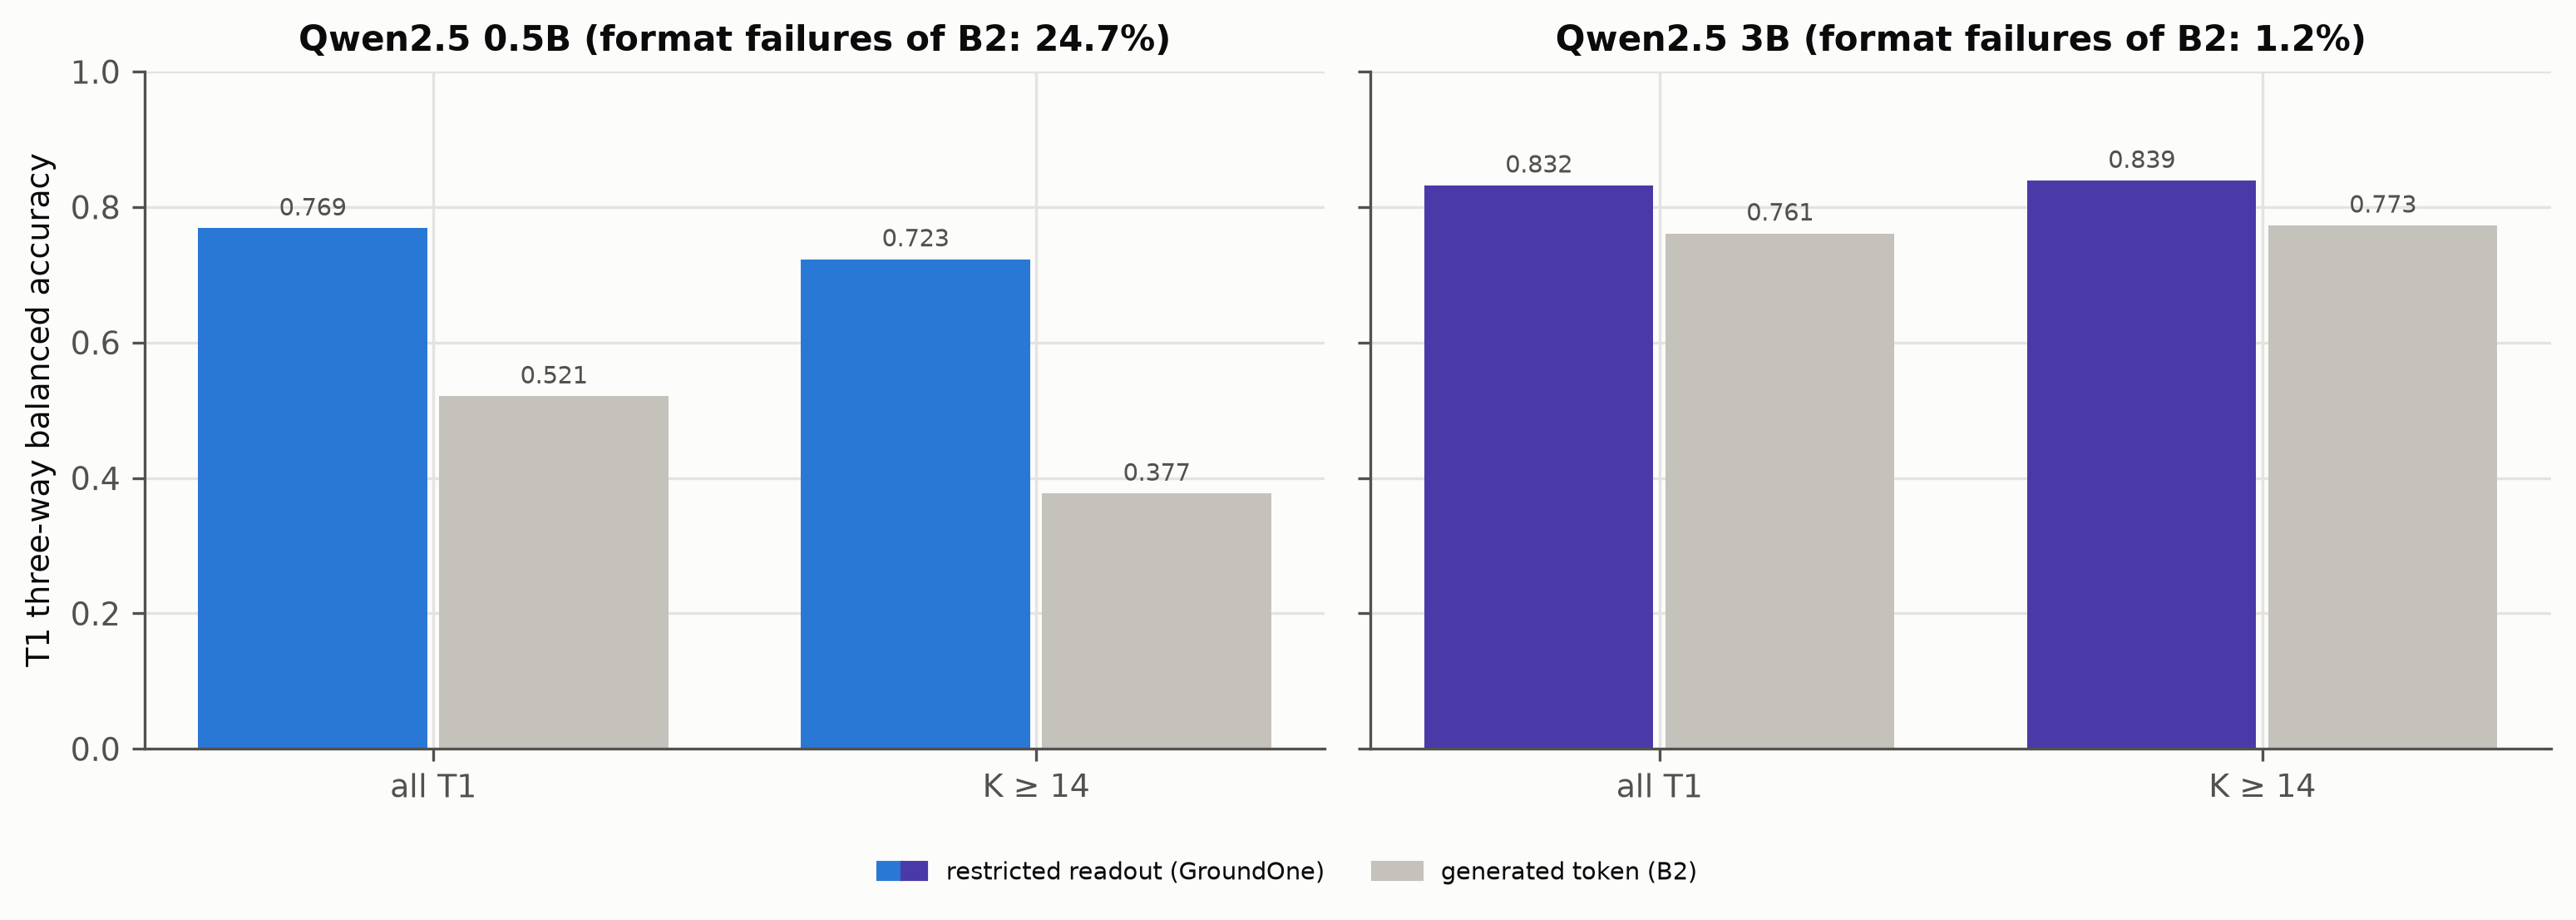
\includegraphics[width=\textwidth]{images/results/readout_vs_generation.png}
\caption{Control B2 on the whole of T1. With the same weights and the same forward pass, the verdict is read from the
three answer letters (GroundOne) or taken as the token that greedy generation would emit; format failures are counted as
errors.}
\label{fig:results-readout}
\end{figure}

The two options have the same latency, because both require a single forward pass: only the decision rule changes.
Restricting the choice to the admissible options removes format failures by construction. Moreover, since the model is
trained only to order the three letters, the restricted choice also provides the more accurate decision
(Section~\ref{sec:method-readout}). This restriction matters all the more, the smaller the model. It is often said that
reading the answer logits and generating a single answer token are equivalent operations: for a fine-tuned verifier the
equivalence holds for the cost, but not for the accuracy.

\section{Calibration and selective prediction}
\label{sec:results-calibration}

Before calibration, the probabilities underestimate support. In the reliability diagram
(Figure~\ref{fig:results-reliability}) the curve of the raw probabilities lies above the diagonal, because the class
weights train the model as if the classes were balanced. The binary ECE on T1 is 0.30 for the 0.5B and 0.18 for the 3B.
The temperature and bias fitted on the dev set bring it to 0.019 for both models, and to 0.020 for the second run of the
0.5B. They also reduce the negative log-likelihood from 0.55 to 0.21 for the 0.5B and from 0.36 to 0.17 for the 3B,
leaving the AUROC practically unchanged. The map fitted on the dev set therefore transfers to the test set of the same
domain. Figure~\ref{fig:results-reliability-3b} shows the same diagram for the 3B.

\begin{figure}[htbp]
\centering
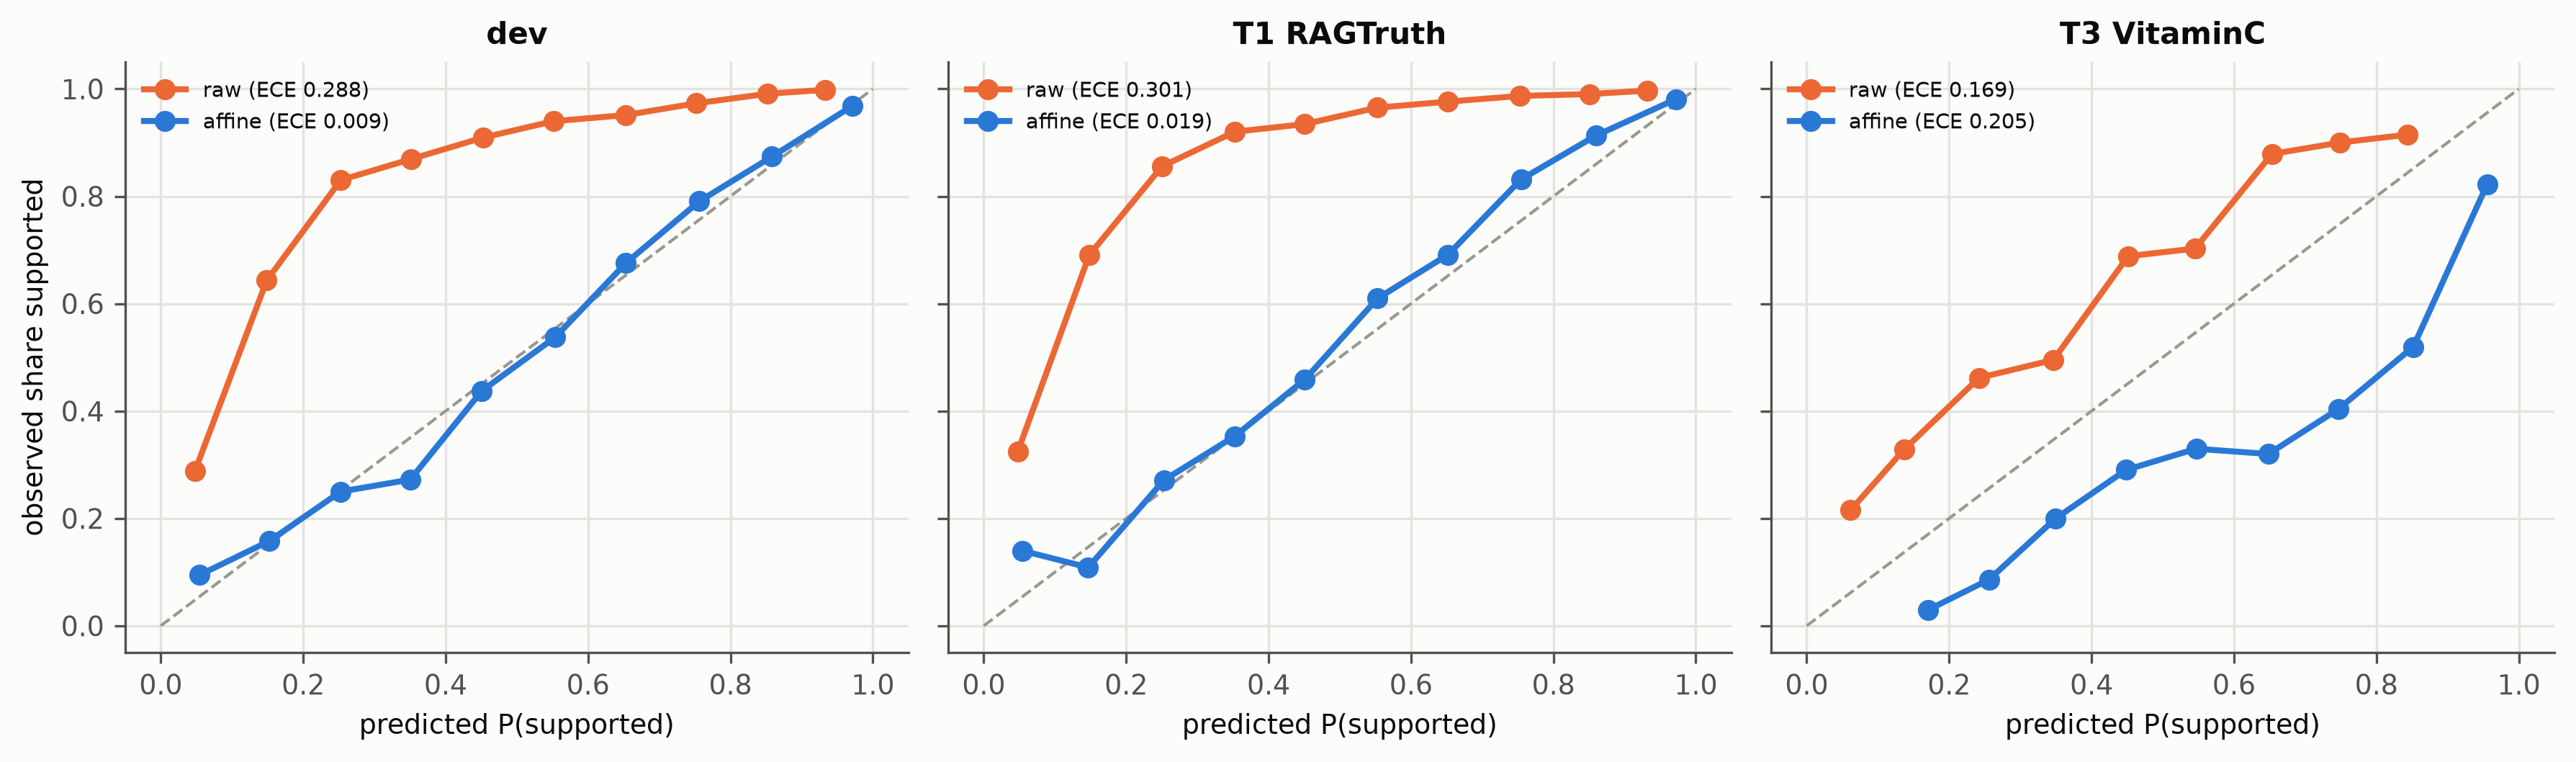
\includegraphics[width=\textwidth]{images/results/g1-05b-reliability.png}
\caption{Reliability diagram of $P(\text{supported})$ of the 0.5B, before calibration (raw) and after the calibration
fitted on the dev set, for the dev set, T1 and T3. Each point represents a probability bin containing at least 20
sentences.}
\label{fig:results-reliability}
\end{figure}

\begin{figure}[htbp]
\centering
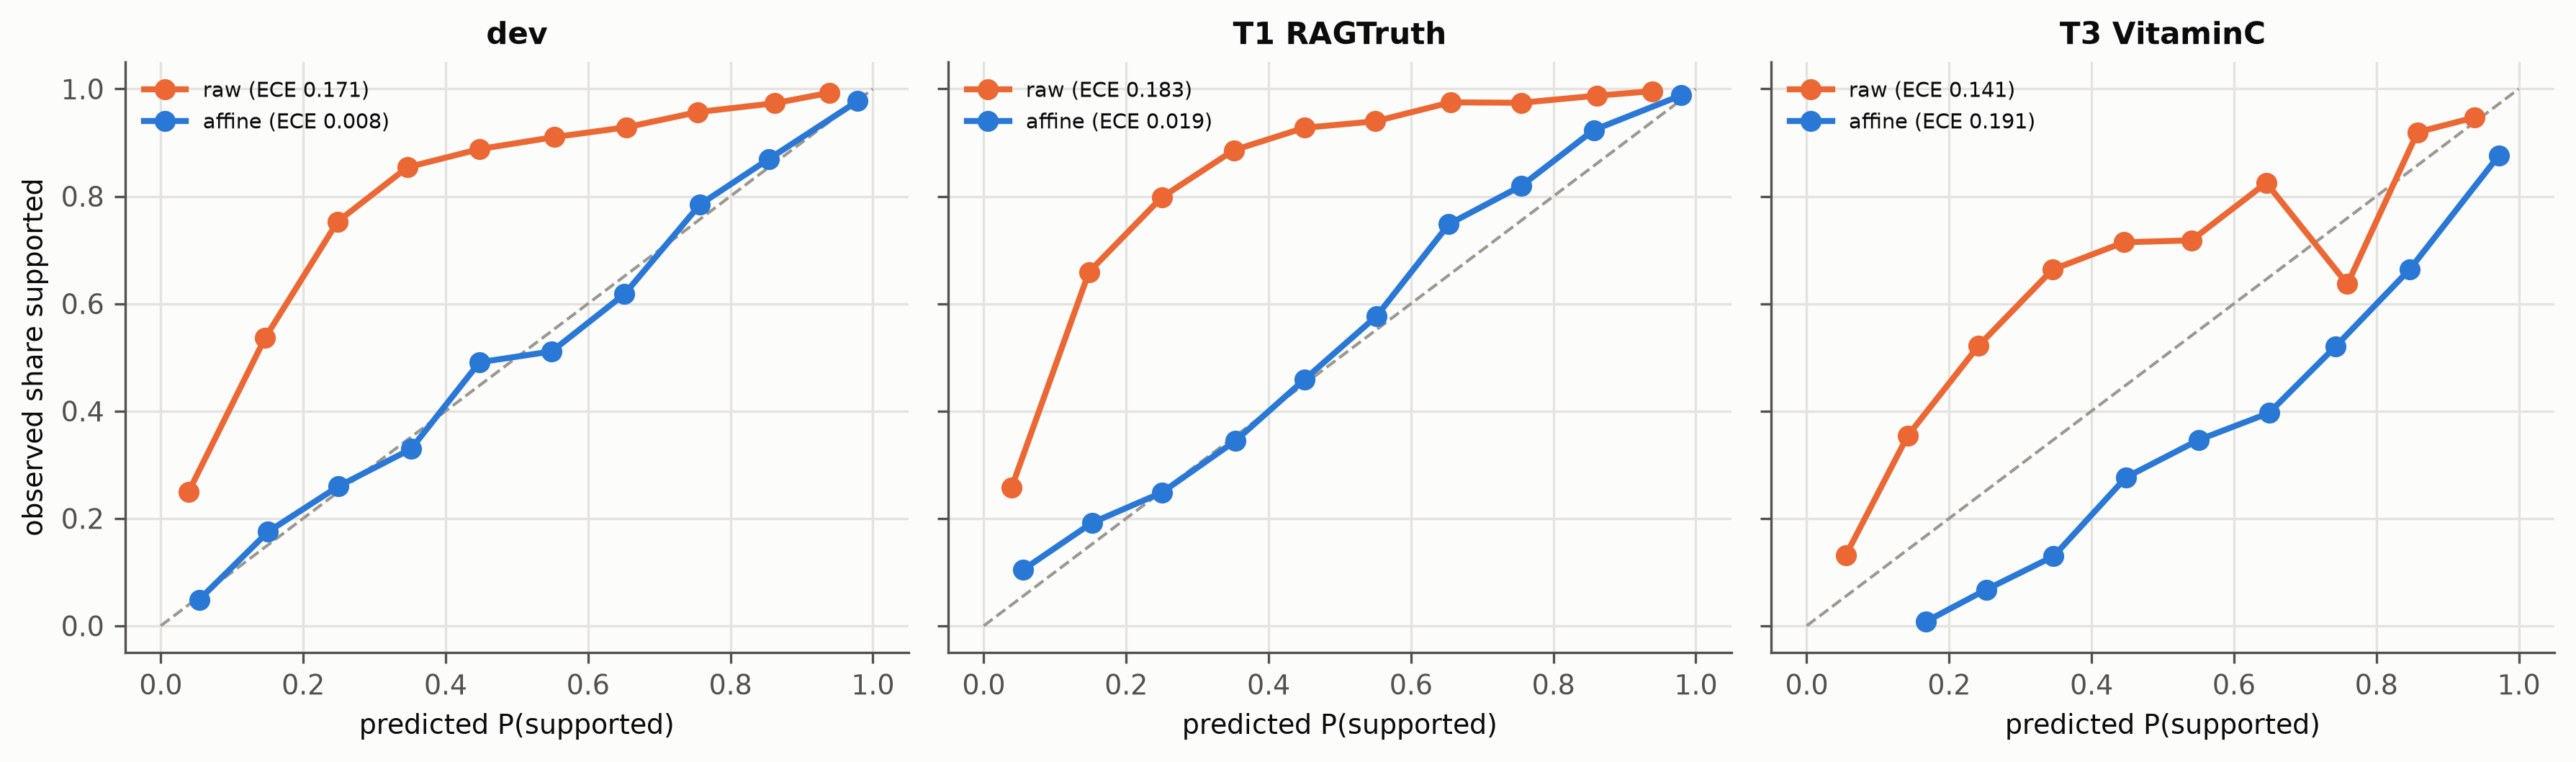
\includegraphics[width=\textwidth]{images/results/g1-3b-reliability.png}
\caption{Reliability diagram of $P(\text{supported})$ of the 3B, before and after the calibration fitted on the dev set, for the dev set, T1 and T3; each point is a probability bin with at least 20 sentences. As for the 0.5B, the calibration transfers to T1 but not to T3.}
\label{fig:results-reliability-3b}
\end{figure}

Calibration, however, has a consequence that must be kept in mind. The bias restores the true frequency of each class,
so the most probable class after calibration becomes ``supported'' more often. For the 0.5B on T1 the accuracy thus
rises from 0.82 to 0.93, but the three-way balanced accuracy falls from 0.77 to 0.63. When the three kinds of error
carry the same weight, therefore, choosing the most probable calibrated class is not a good decision rule. The rule with
which the labels are served, described in Section~\ref{sec:method-calibration}, solves the problem. The rule uses a
threshold $\tau$ fitted on the dev set, equal to 0.935 for the 0.5B, to 0.895 for its second run and to 0.925 for the
3B. With these thresholds it reaches on T1 a three-way balanced accuracy of 0.758, 0.769 and 0.830, within about 0.01 of
the raw decision evaluated throughout the chapter, and keeps the labels consistent with the calibrated probabilities.
The thresholds are high because about 88\,\% of the sentences of the training and dev sets are supported: a sentence is
served as supported only when the model is very confident.

Used as confidences, the calibrated probabilities make selective prediction effective. Deferring the sentences on which
the model is least confident quickly reduces the error rate of the binary decision: on T1 the AURC is 0.015 for the 0.5B
and 0.010 for the 3B (Figure~\ref{fig:results-risk}).

\begin{figure}[htbp]
\centering
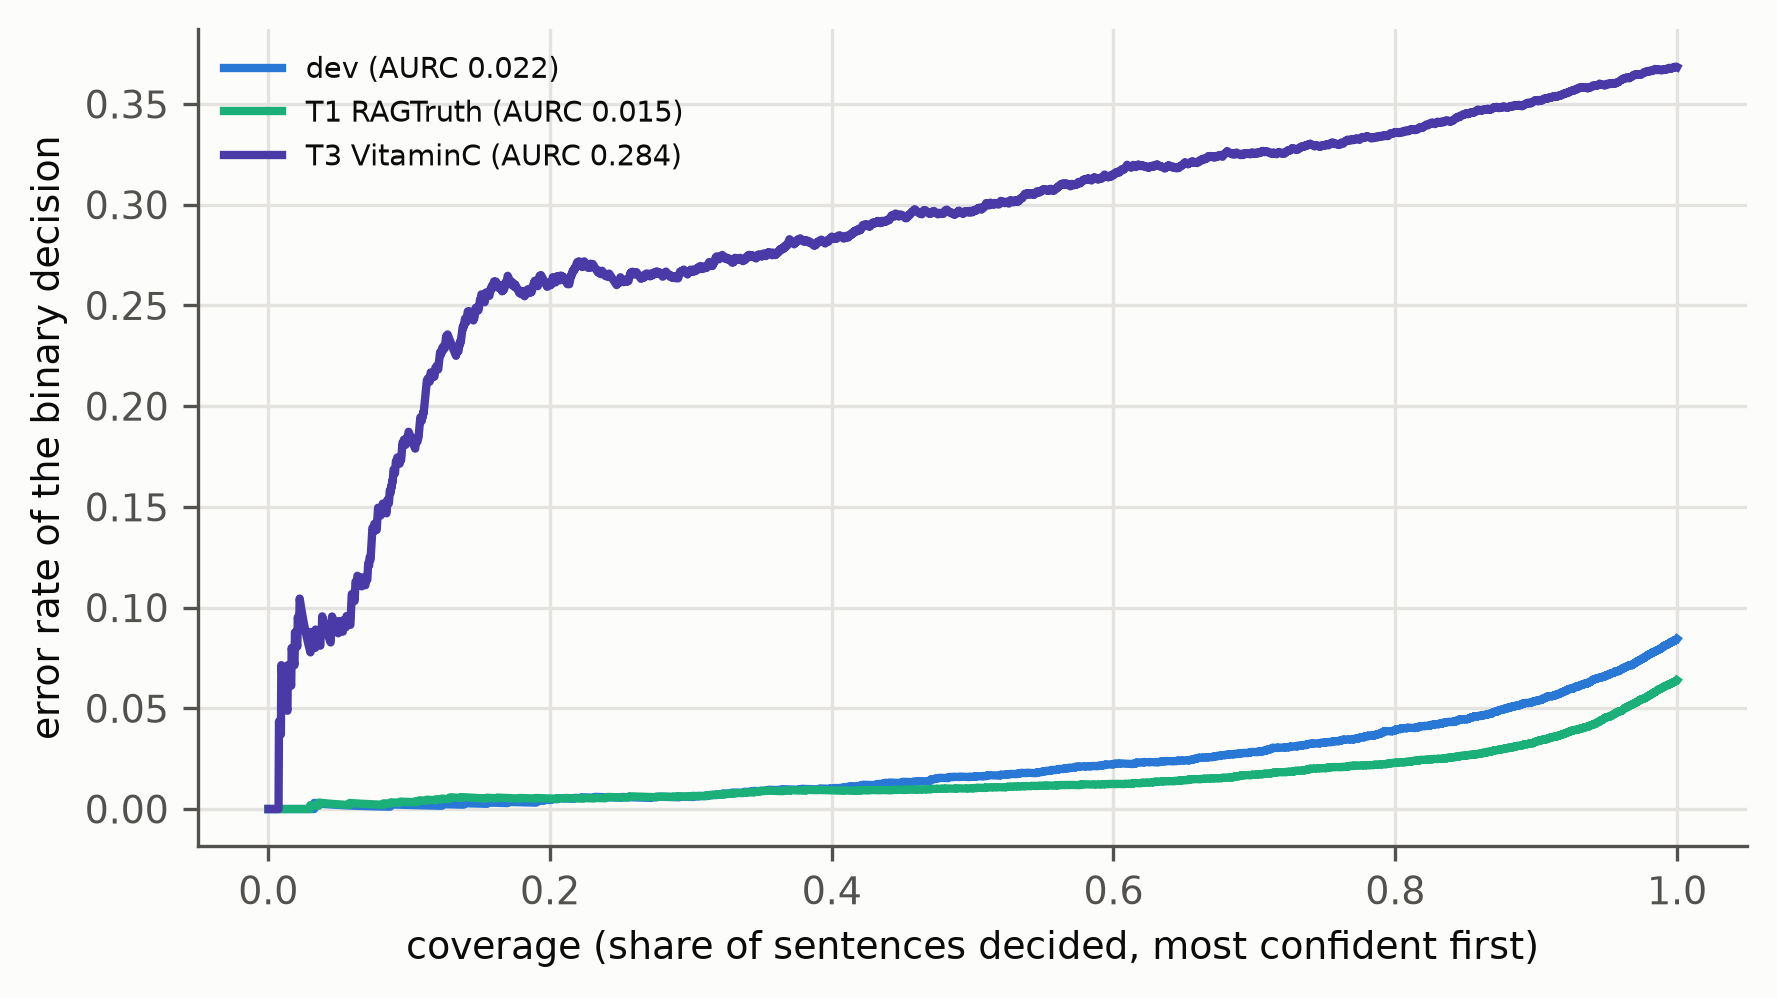
\includegraphics[width=0.75\textwidth]{images/results/g1-05b-risk_coverage.png}
\caption{Risk--coverage curves of the binary decision of the 0.5B with calibrated probabilities: error rate as the
number of least confident sentences that are deferred grows.}
\label{fig:results-risk}
\end{figure}

On VitaminC, instead, the calibration does not transfer. The binary ECE rises from 0.17 to 0.21 for the 0.5B and from
0.14 to 0.19 for the 3B, and the rule with which the labels are served loses 0.02--0.04 with respect to the raw
decision. The bias, in fact, encodes the base rate of RAGTruth, whereas VitaminC is balanced by construction. A
calibration holds for the distribution on which it was fitted, so every real deployment requires a small labelled
sample of its own data.

\section{Probabilities at equal output}
\label{sec:results-equal-output}

The equal-output LLM judges serve to establish whether an LLM judge of the same size, asked for the same content as
GroundOne, can match the quality of its probabilities. The answer is negative (Figure~\ref{fig:results-equal}). The
comparison uses the 200 answers of the latency subset, with all systems calibrated in the same way on the dev set. For
the 0.5B and the 3B respectively, the AUROC of $P(\text{supported})$ is 0.94 and 0.97 for GroundOne, 0.48 and 0.68 for
the LLM judge whose probabilities are read from the logits, and 0.47 and 0.58 for the LLM judge that writes them. The AURC is
0.009 and 0.005 for GroundOne, against values from 0.048 to 0.063 for the LLM judges, that is, about seven to twelve times
larger than those of GroundOne of the same size. The accuracy of the decisions follows the same pattern: 0.835 and 0.900
for GroundOne, at most 0.41 for any LLM judge.

\begin{figure}[htbp]
\centering
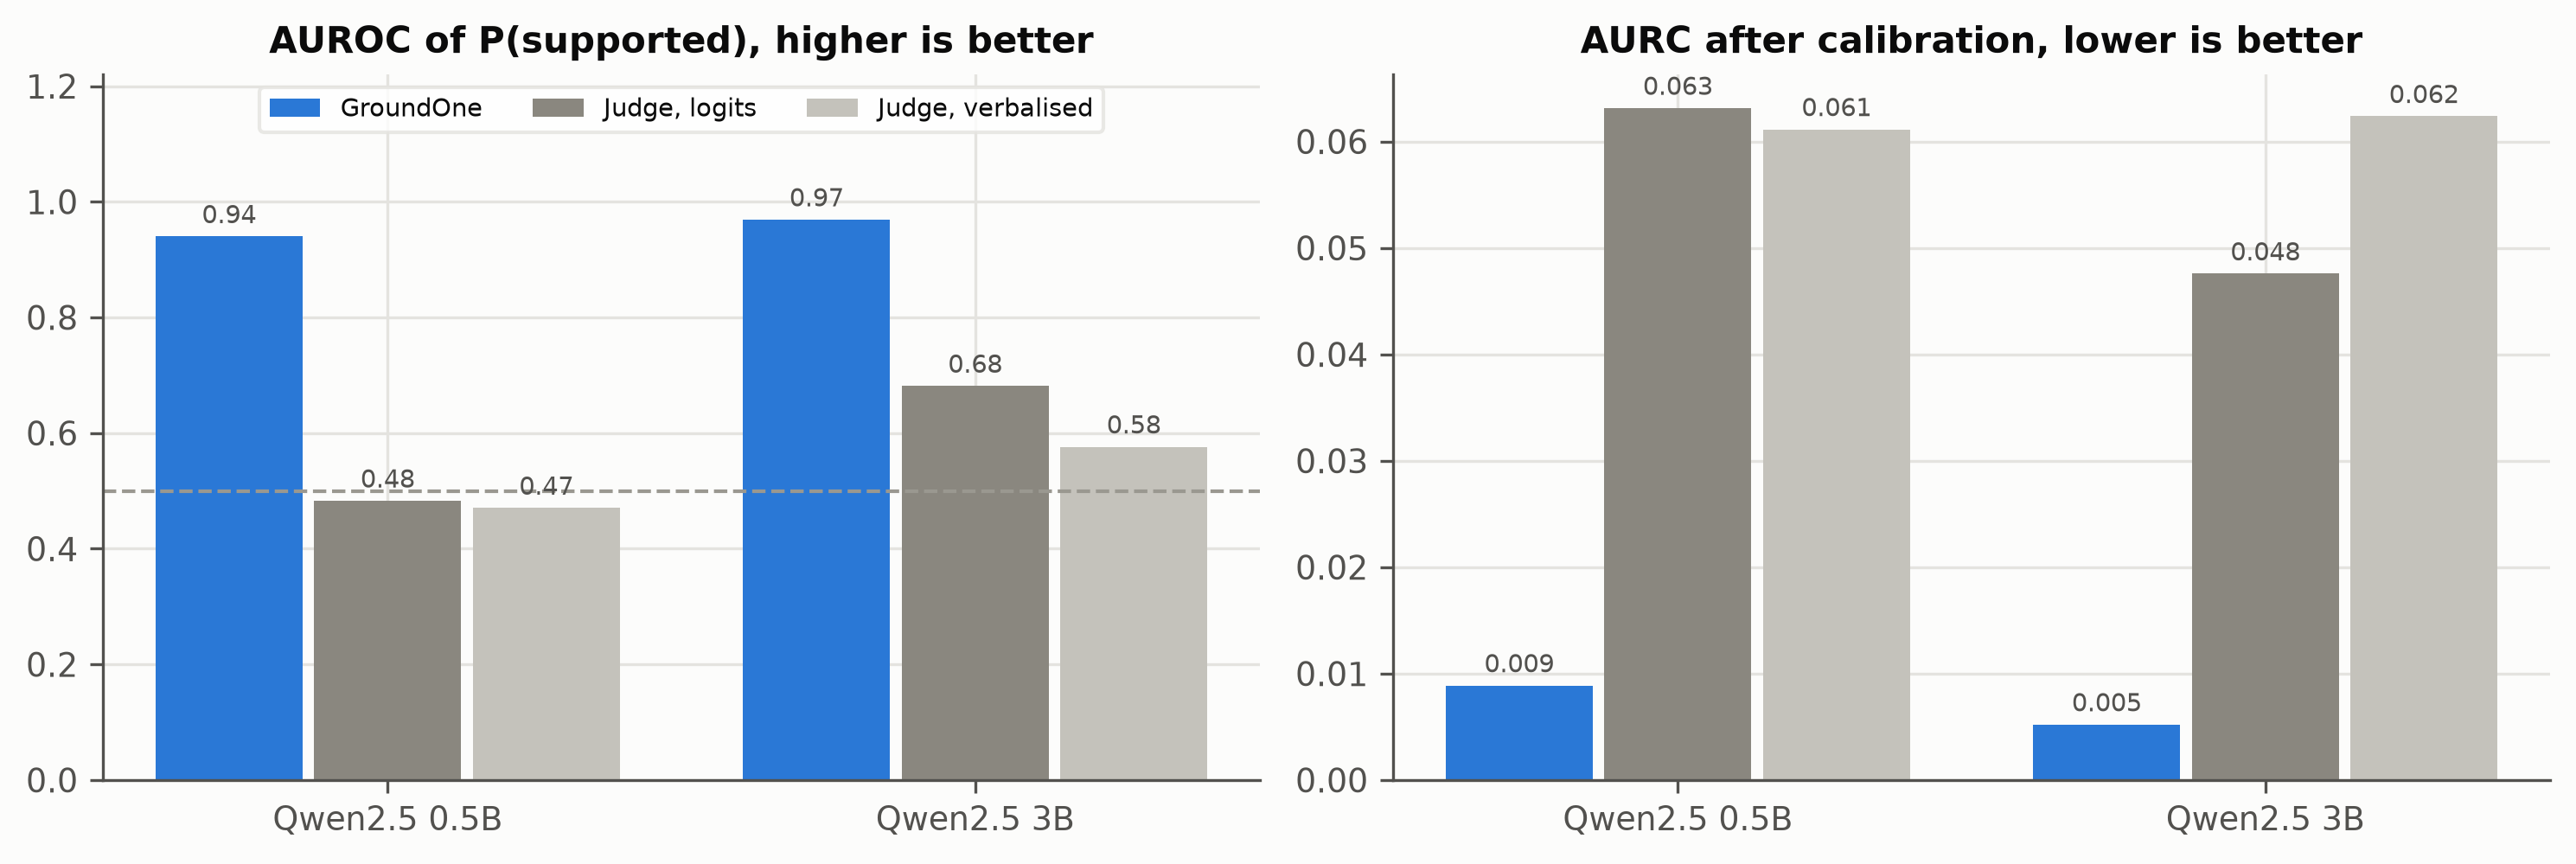
\includegraphics[width=\textwidth]{images/results/equal_output_judges.png}
\caption{Equal-output comparison on the 200 answers of the latency subset. LLM judges of the same size are asked
for GroundOne's output, with the probabilities read from the logits of the generated letter or written in JSON; all
systems are calibrated on the dev set with the same map. Only the sentences with a valid verdict are considered.}
\label{fig:results-equal}
\end{figure}

Two further observations matter in practice. The first is that probabilities written in words carry almost no
information. The 3B writes a vector with all the mass on a single class for 93\,\% of the sentences, and uses only
sixteen distinct vectors. The 0.5B instead writes uninformative ties, such as equal probabilities for all classes: if
the ties without a label are counted as errors, its balanced accuracy falls from 0.234 to 0.081. This agrees with the
observation that the verbalised confidence of small models is coarse and poorly
informative~\cite{xiong2024uncertainty,tian2023justask}. The second observation is that the ECE alone would hide all of
this. After calibration every system, LLM judges included, obtains a binary ECE between 0.03 and 0.05, because a
calibration map can align the average confidence with the base rate even when the probabilities do not separate the
classes. Discriminative ability must therefore be measured separately, with the AUROC and the AURC.

Asking for the probabilities, finally, has a cost. The LLM judge that reads them from the logits is as fast as the terse
LLM judge, because it generates the same letters. The LLM judge that writes the JSON object, instead, needs 17.0 seconds with
the 3B for an answer with fourteen or more decisions, as much as the verbose LLM judge, and is no more accurate than the
terse LLM judge.

\section{Latency as a function of $K$}
\label{sec:results-latency}

Figure~\ref{fig:results-latency} reports the central measurement of the thesis: the time needed to verify an answer as
the number of decisions grows, measured on the same 200 answers of T1. Among the systems run in process on MLX,
GroundOne is the fastest at both sizes and in every band of $K$, and its advantage grows with $K$. When the answer
contains fourteen or more decisions, the 0.5B GroundOne needs 0.41 seconds, against 0.80 for the terse LLM judge and 2.51
for the verbose LLM judge of the same size. It is therefore 1.95 times faster than the first (1.82 to 2.12) and 6.16 times
faster than the second (5.72 to 6.66). In the same band the 3B GroundOne needs 2.57 seconds, against 4.44 and 15.86
seconds for the two 3B LLM judges, and is therefore 1.73 times (1.65 to 1.82) and 6.18 times (5.88 to 6.63) faster.

Reading all the verdicts in a single forward pass is also faster than asking one question per sentence in a batch: at
the highest values of $K$ the gain is a factor of 1.4--1.5. The other lever is model size: the 0.5B GroundOne verifies
an answer about six times faster than the 3B, with a median time of 0.33 seconds against 1.99.

\begin{figure}[htbp]
\centering
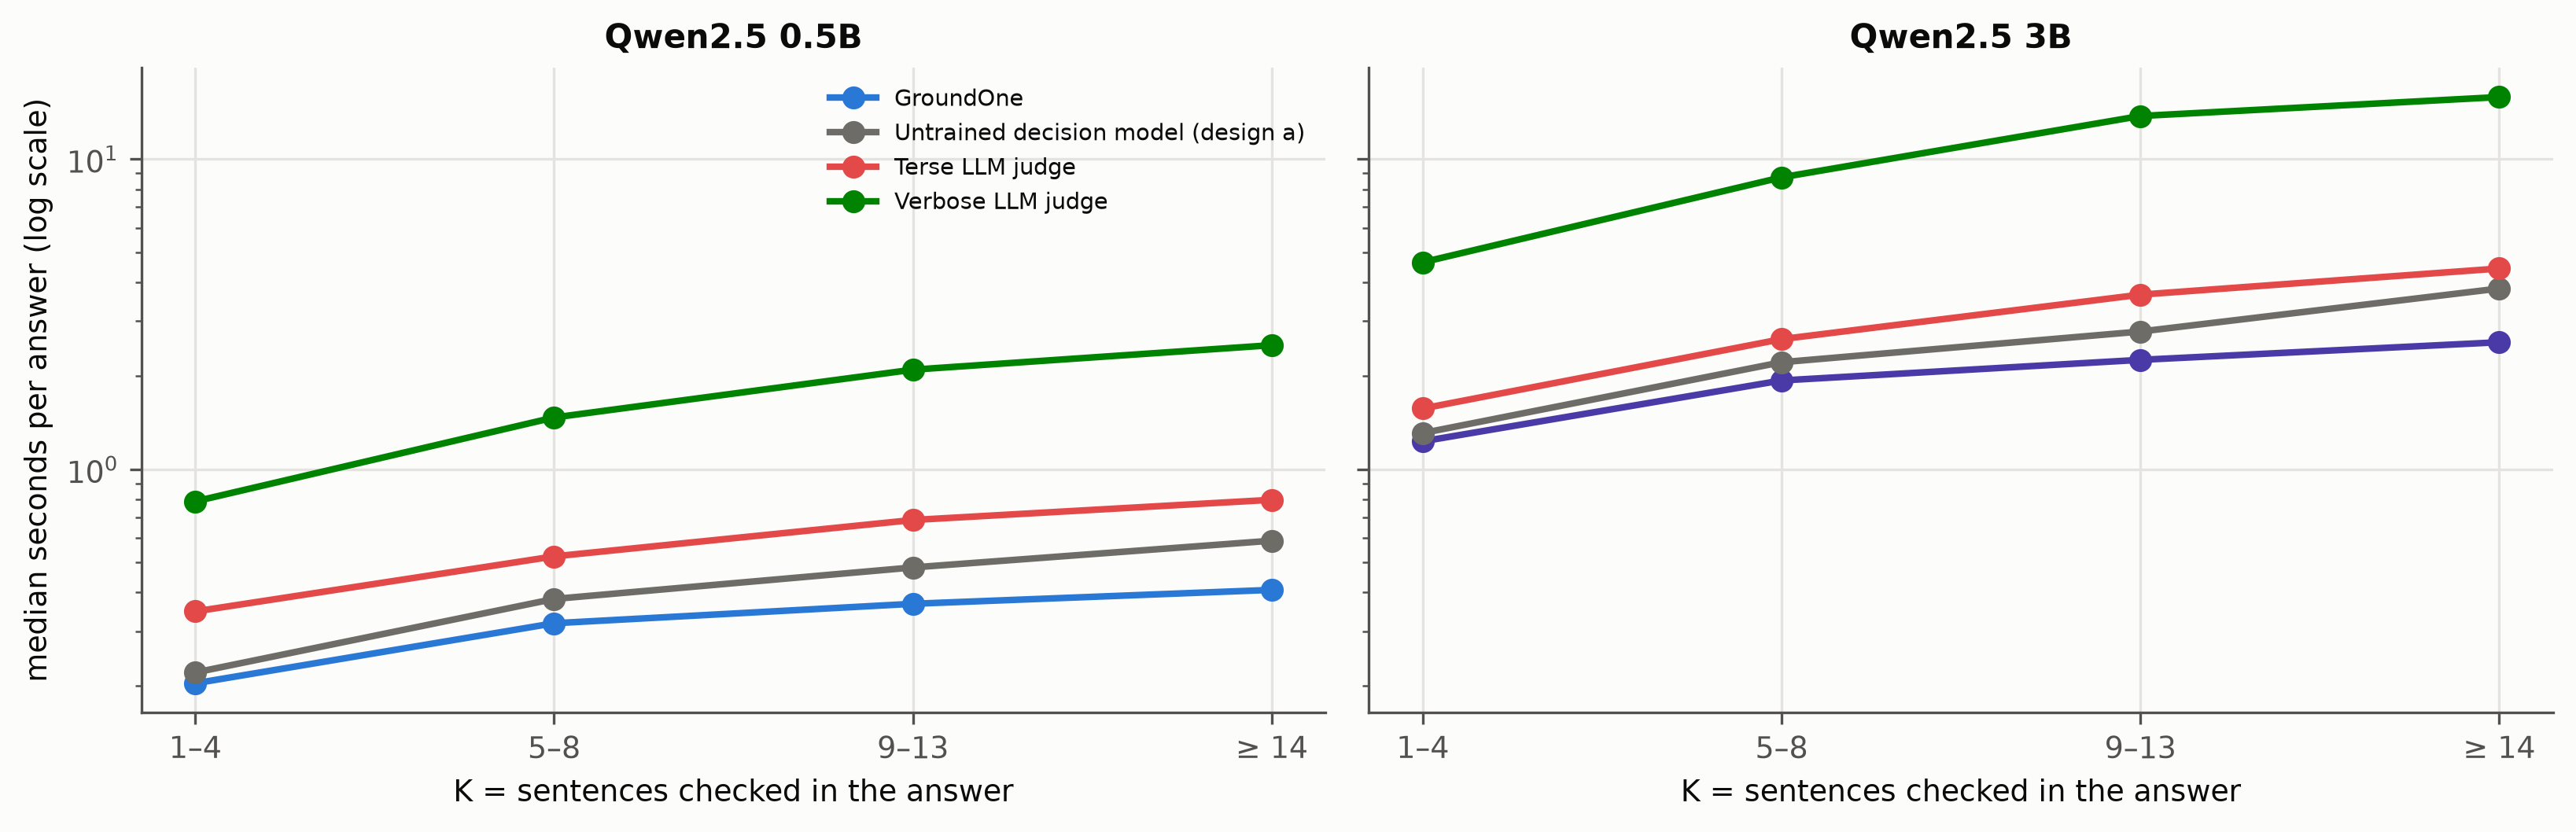
\includegraphics[width=\textwidth]{images/results/latency_vs_K.png}
\caption{Median time per answer as a function of $K$ on the same 200 answers of T1 (in-process MLX, one answer at a
time, M4 with 16\,GB). GroundOne, the decision model with one question per sentence and the terse and verbose
LLM judges are compared. Logarithmic scale.}
\label{fig:results-latency}
\end{figure}

\subsection{Reading the text and deciding}
\label{sec:results-latency-split}

GroundOne's time grows with $K$, but not because of the number of decisions as such. Answers with more sentences are
also longer: in the latency subset the prompt goes from about 550 tokens in the $K \leq 4$ band to about 1{,}140 tokens
at $K \geq 14$, and the prefill time grows with the length of the text. To separate the two components, the time of
every answer was split into a \emph{reading} part, the prefill of instructions, document and answer that every approach
must pay, and a \emph{deciding} part. For GroundOne, reading is a forward pass over the same text without markers, and
deciding is the difference from the served pass, that is, the cost of the markers and of the readout; the two
measurements are interleaved five times with the 0.5B and three times with the 3B, and the median is kept. For the LLM
judges, reading is the time to the first generated token, and deciding is the decoding of the verdicts. The measurement
uses the same 200 answers and the same protocol as the previous section, and reproduces its overall times within
4\,\%. Table~\ref{tab:results-latency-split} reports the medians, Figure~\ref{fig:results-latency-split} their trend
with $K$.

\begin{table}[htbp]
\centering
\caption{Time per answer split into reading the text (prefill) and deciding, on the same 200 T1 answers: medians over
all answers, in seconds. For GroundOne deciding is the cost of the markers and of the readout, for the LLM judges the
decoding of the verdicts. The reading share is the median of the per-answer shares.}
\label{tab:results-latency-split}
\small
\begin{tabular}{llcccc}
\toprule
Model & System & Reading & Deciding & Total & \makecell{Reading\\share} \\
\midrule
0.5B & GroundOne & 0.330 & 0.012 & 0.342 & 97\,\% \\
 & Terse LLM judge & 0.297 & 0.383 & 0.673 & 46\,\% \\
 & Verbose LLM judge & 0.305 & 1.509 & 1.826 & 18\,\% \\
\midrule
3B & GroundOne & 1.941 & 0.067 & 2.002 & 97\,\% \\
 & Terse LLM judge & 1.753 & 1.196 & 3.102 & 61\,\% \\
 & Verbose LLM judge & 1.756 & 8.313 & 10.277 & 18\,\% \\
\bottomrule
\end{tabular}
\end{table}

For GroundOne, reading takes 97\,\% of the time at both sizes. Deciding costs a median of 12 milliseconds per answer
with the 0.5B and 67 with the 3B, that is, 1.3 and 6.7 milliseconds per sentence: the three tokens of the marker and the
vocabulary projection at the marker positions only. The terse LLM judge spends instead 30 and 139 milliseconds per
sentence, the verbose one 170 and 1{,}033. For the LLM judges, deciding is a substantial part of the time, and for the
verbose LLM judge the main part. Net of reading, GroundOne decides 33 times faster than the terse LLM judge with the 0.5B
(30 to 38) and 18 times faster with the 3B (15 to 20); against the verbose LLM judge, 131 times (112 to 148) and 125
times (116 to 142). With fourteen or more sentences the ratios are similar: 29 and 24 times against the terse LLM judge,
141 and 151 against the verbose one.

The overall speed-up remains about two against the terse LLM judge because reading, which dominates the time, is shared by
all approaches: GroundOne's advantage lies in the part that the readout replaces, not in the prefill. The split also
shows a cost that the overall times hide. GroundOne's reading is about 10\,\% slower than that of the LLM judges,
although its prompt is slightly shorter: it is the extra computation of the LoRA adapter, which stays separate from the
quantised base weights. Fusing the adapter into the weights would remove this cost, but would require quantising the
model again and recalibrating it.

\begin{figure}[htbp]
\centering
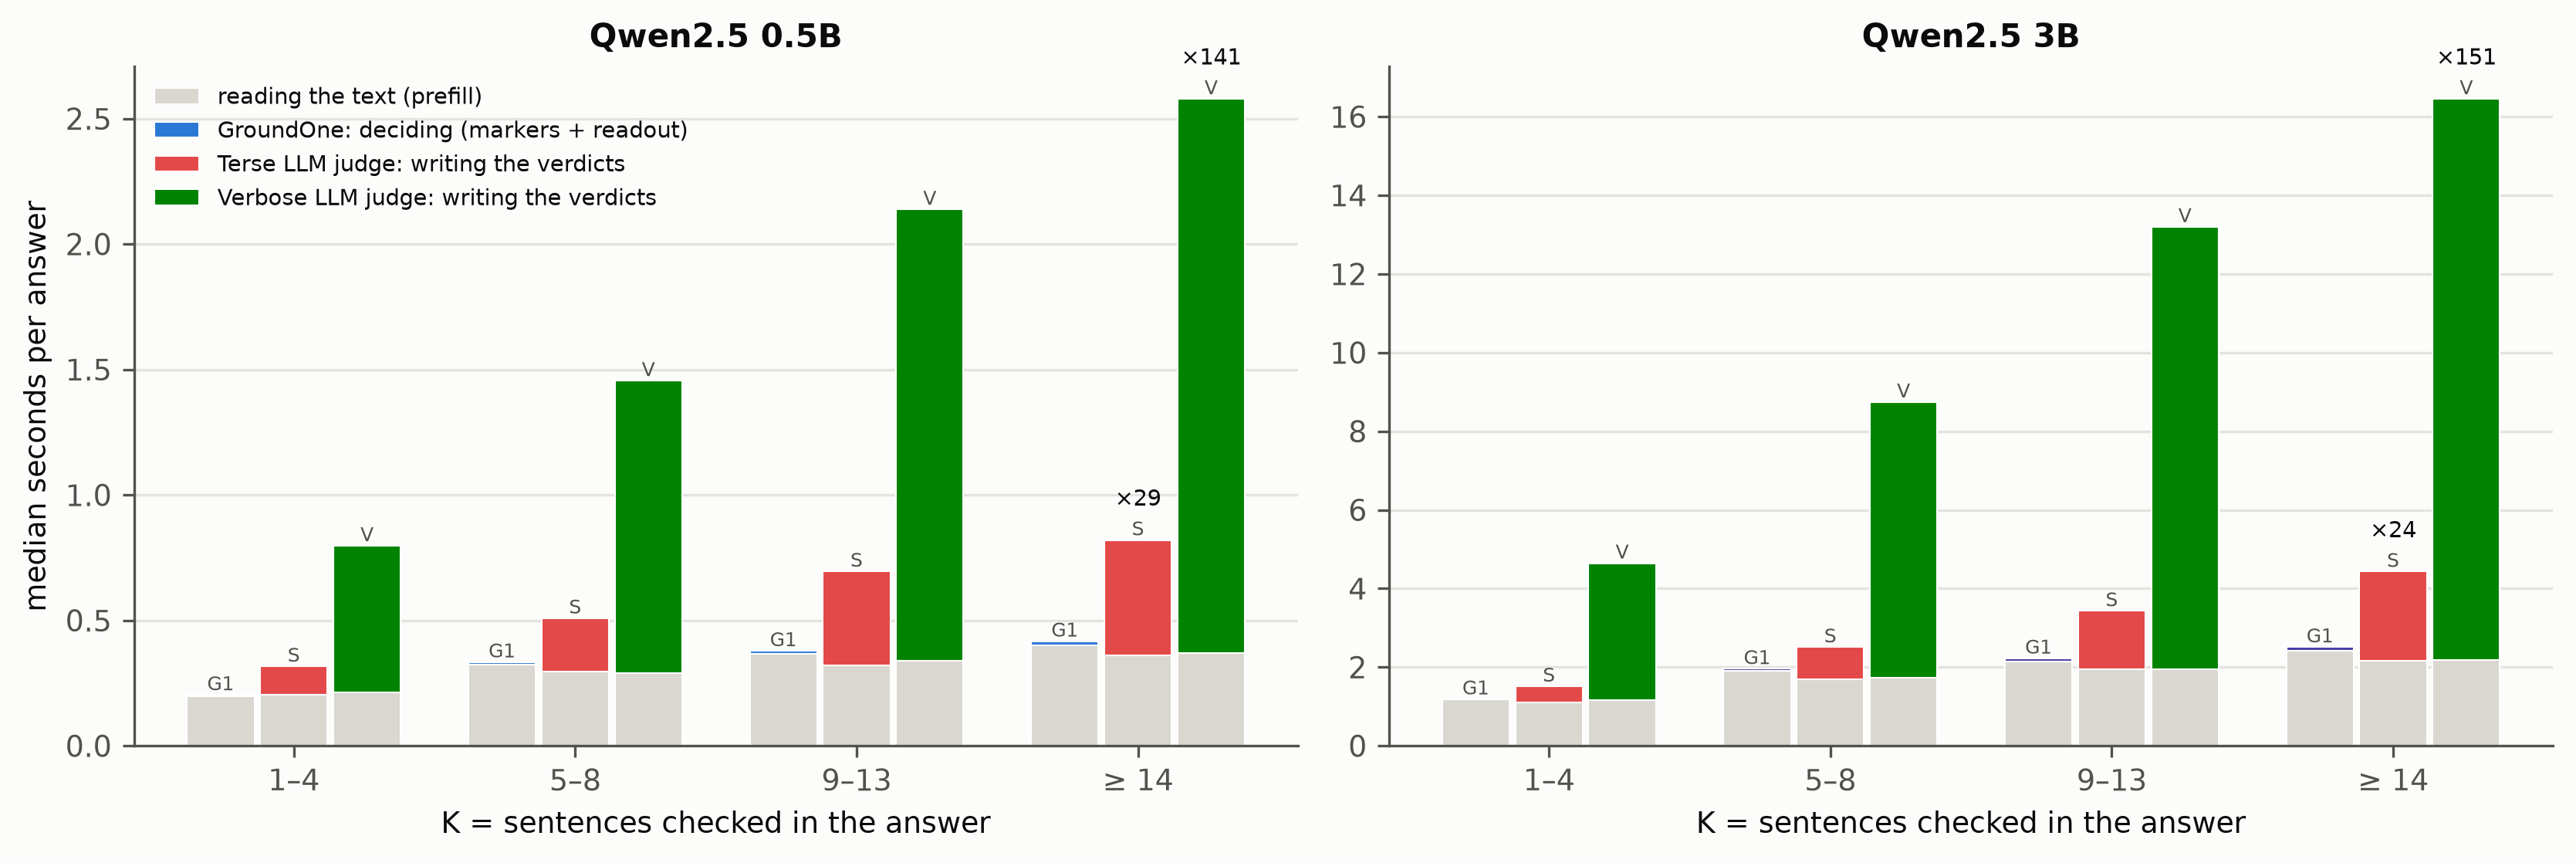
\includegraphics[width=\textwidth]{images/results/latency_split.png}
\caption{Median time per answer split into reading the text (prefill, in grey, shared by every approach) and deciding
(in colour), per $K$ band, on the same 200 T1 answers. The labels give, for $K \geq 14$, how many times longer the LLM
judge takes to decide than GroundOne.}
\label{fig:results-latency-split}
\end{figure}

\paragraph{Prefix reuse.} The same measurement was repeated with part of the prompt already in the KV cache when the
clock starts, the same for GroundOne and for the LLM judges: the instructions alone, identical for every request (63 to
81 tokens), or the instructions and the document (about 640 tokens at the median), as when a rewritten answer is
verified again on the same sources (Section~\ref{sec:method-readout}).\footnote{In the MLX version used for the
measurements (0.29.3), the fused attention kernel with the implicit causal mask returns wrong results for some shapes
when many queries follow cached keys, for example 501 tokens read after 523 cached ones. The paths with a cached prefix
therefore use an explicit causal mask, which matches a float32 reference; after this correction the logits with and
without the cache differ by at most 0.07 and the probabilities by 0.014, that is, within bfloat16 rounding. The
measurements without a cache, and so all the other results, do not take this path. The Swift version of MLX used by the
application does not show the error.} Table~\ref{tab:results-prefix-cache} reports the overall times.

\begin{table}[htbp]
\centering
\caption{Overall time per answer with part of the prompt already in the KV cache, on the same 200 T1 answers: medians
in seconds. The same cache applies to GroundOne and to the LLM judges. The last column is the ratio between the median
times without a cache and with the document cached.}
\label{tab:results-prefix-cache}
\small
\setlength{\tabcolsep}{4pt}
\begin{tabular}{llcccc}
\toprule
Model & System & \makecell{No\\prefix} & \makecell{Instructions\\cached} & \makecell{Document\\cached} & \makecell{Saving with\\the document} \\
\midrule
0.5B & GroundOne & 0.342 & 0.333 & 0.108 & 3.2$\times$ \\
 & Terse LLM judge & 0.673 & 0.652 & 0.520 & 1.3$\times$ \\
 & Verbose LLM judge & 1.826 & 1.844 & 1.683 & 1.1$\times$ \\
\midrule
3B & GroundOne & 2.002 & 1.913 & 0.583 & 3.4$\times$ \\
 & Terse LLM judge & 3.102 & 3.002 & 1.795 & 1.7$\times$ \\
 & Verbose LLM judge & 10.277 & 9.998 & 8.742 & 1.2$\times$ \\
\bottomrule
\end{tabular}
\end{table}

Caching the instructions alone saves 3 to 5\,\% of the time, little more than the measurement noise: they are 7\,\% of
the tokens. The document, instead, is about two thirds of the prompt, and the difference is clear. With the document
cached, GroundOne verifies an answer 3.2 times faster with the 0.5B (0.11 seconds at the median) and 3.4 times faster
with the 3B (0.58 seconds). The LLM judges gain much less, 1.3 and 1.7 times for the terse one and 1.1 and 1.2 for the
verbose one, because the cache removes only the reading and leaves the decoding of the verdicts intact, which cannot be
reused. As a result, GroundOne's advantage over the terse LLM judge rises from about 2 to 4.8 times with the 0.5B (4.1
to 5.2) and from 1.6 to 3.1 times with the 3B (2.8 to 3.3), and over the verbose LLM judge to about 15 times. With the
document cached, 90\,\% of GroundOne's time is the reading of the answer alone and the rest is deciding: verifying a
rewritten answer therefore costs little more than its length.

Speed is not the only difference (Figure~\ref{fig:results-judges}). The untrained LLM judges are also much less
accurate, and they do not always respect the output format. The 0.5B verbose LLM judge produces a parsable verdict for only
3\,\% of the sentences, because it mostly copies the answer back, while the 0.5B terse LLM judge fails on 23\,\% of the
sentences. The 3B LLM judges respect the format much better (0.1\,\% format failures for the terse LLM judge and 7.6\,\% for the
verbose one), but stop at a three-way balanced accuracy of about 0.40, against 0.90 for the 3B GroundOne on the same
answers. The 3B verbose LLM judge, finally, writes on average 248 tokens per answer, all of which must be generated before
the verdict can be used; GroundOne, instead, generates none.

\begin{figure}[htbp]
\centering
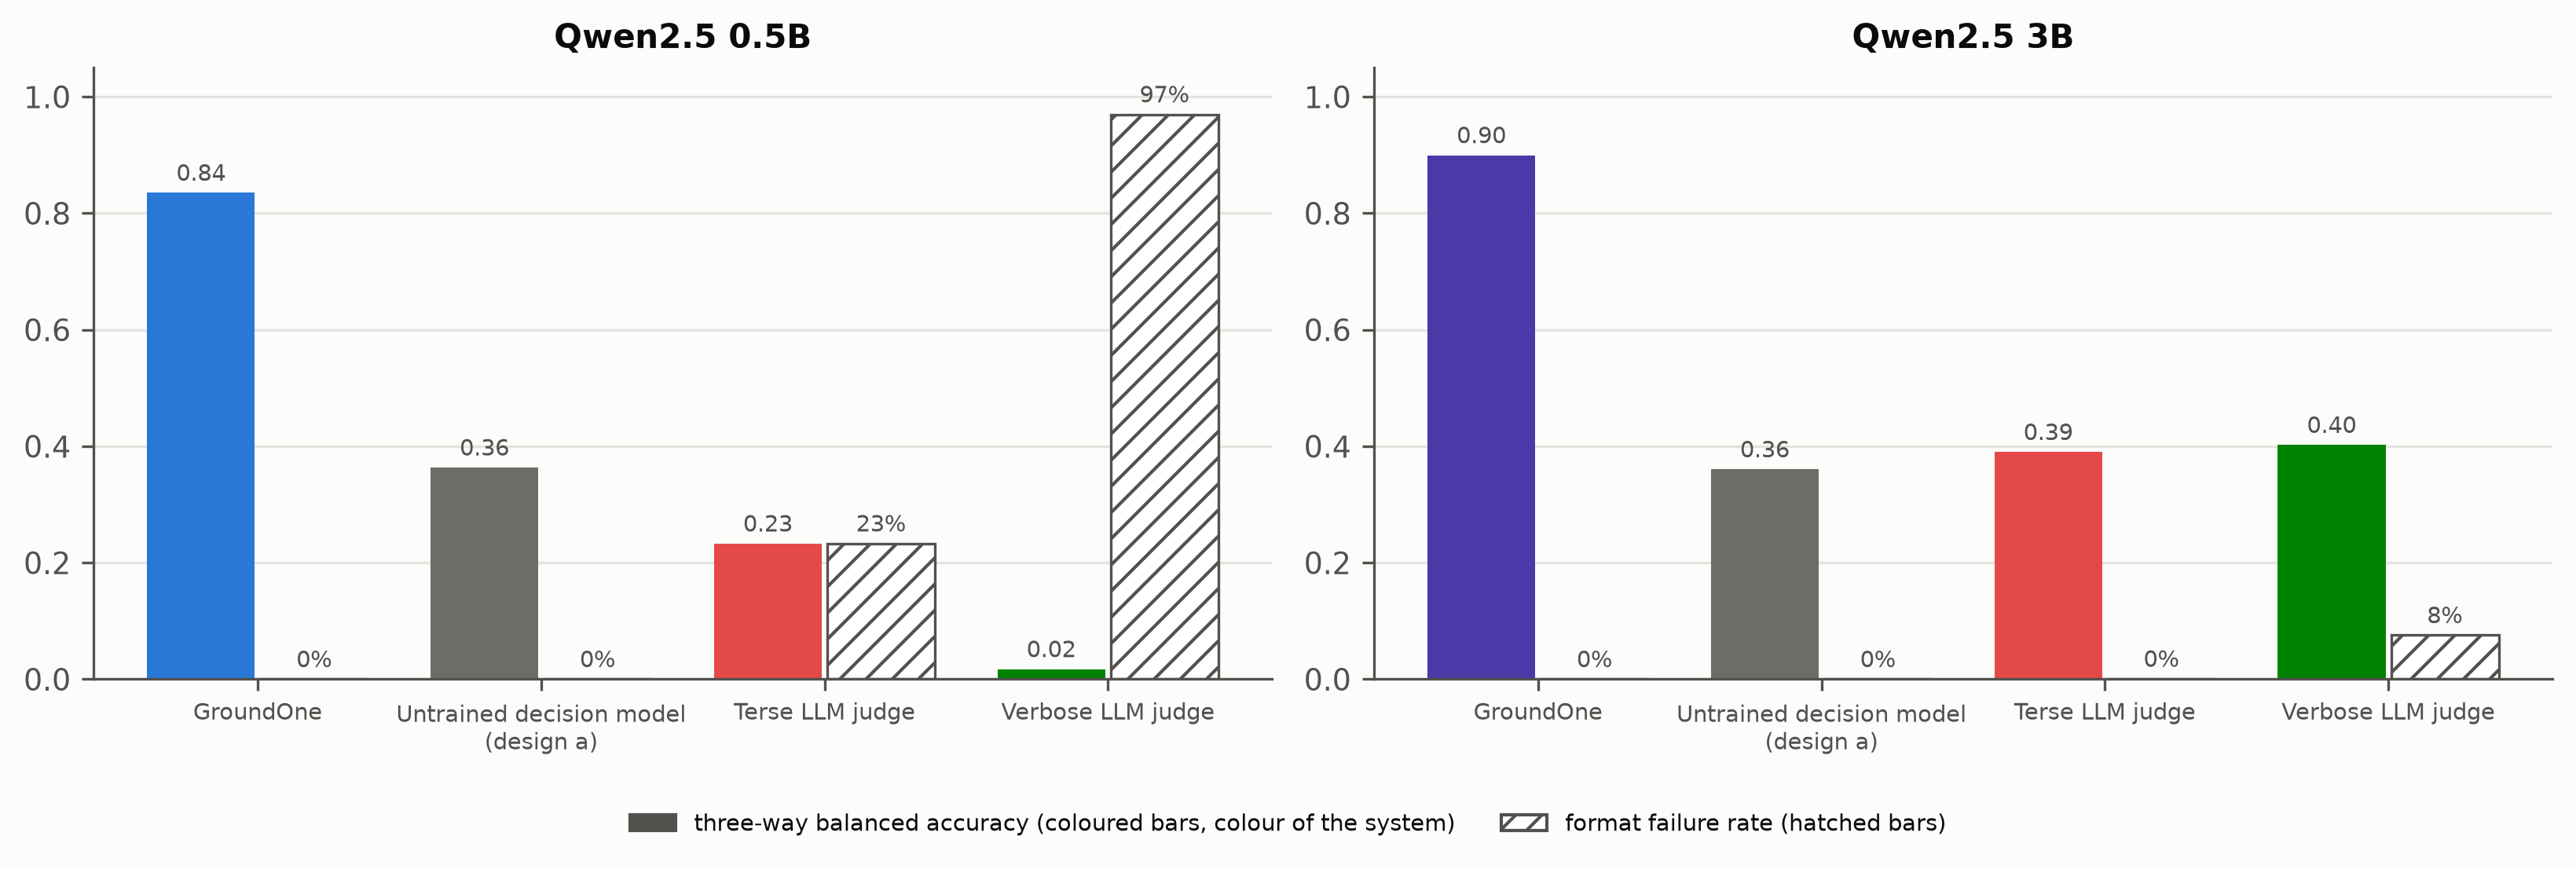
\includegraphics[width=\textwidth]{images/results/judges_quality_failures.png}
\caption{LLM judges on the latency subset: three-way balanced accuracy, with format failures counted as errors,
and share of sentences whose verdict could not be parsed.}
\label{fig:results-judges}
\end{figure}

\section{Energy per verification}
\label{sec:results-energy}

The energy measurement adds a qualification that latency alone hides (Figure~\ref{fig:results-energy}). Among the
measured systems, that is, GroundOne and the LLM judges, GroundOne is the one that uses the least energy at both
sizes: 5.5 joules per answer with the 0.5B and 33 with the 3B, against 8.9 and 43 joules for the terse LLM judge and 22.5
and 112 joules for the verbose LLM judge. Its advantage in energy, however, is smaller than its advantage in time. Compared
with the terse LLM judge, GroundOne uses 1.6 times less energy with the 0.5B and 1.3 times less with the 3B; compared with
the verbose LLM judge, 4.1 and 3.4 times less.

The reason is the power drawn during the computation. GroundOne spends its time in a single long prefill, which keeps
the GPU fully busy and draws about 16\,W above the idle power. The autoregressive decoding of the LLM judges, instead, is
limited by memory bandwidth and draws 11--14\,W, but for a much longer time. This is the behaviour expected from the two
phases of transformer inference~\cite{patel2024splitwise}, and it implies that a speed-up should never be read as an
equivalent saving of energy~\cite{samsi2023words,luccioni2024power}.

\begin{figure}[htbp]
\centering
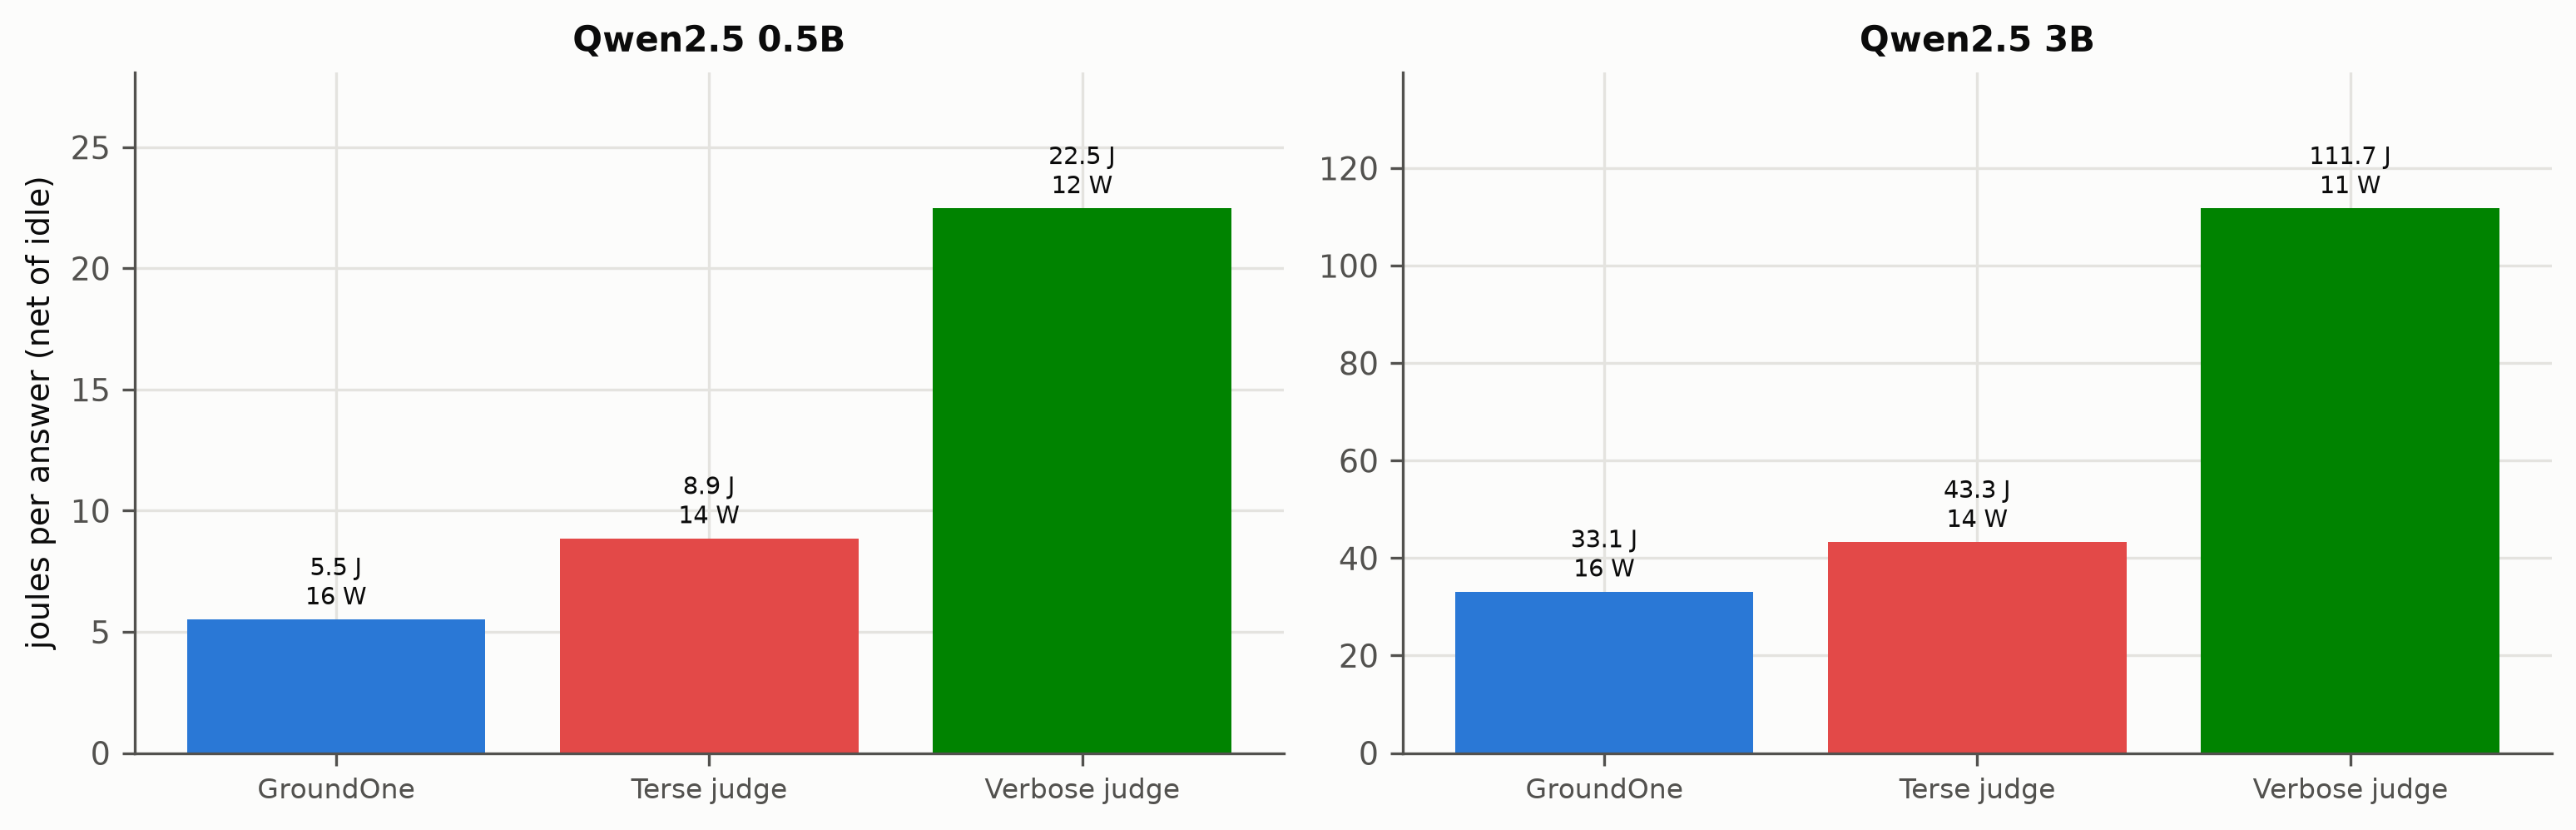
\includegraphics[width=\textwidth]{images/results/energy_per_answer.png}
\caption{Energy per verified answer on 100 answers of the latency subset, measured with \texttt{powermetrics} on the
CPU, GPU and Neural Engine net of the idle power, together with the mean net power during the run.}
\label{fig:results-energy}
\end{figure}

In absolute terms the values are small. A consumption of 5.5 joules corresponds to about 0.0015 watt-hours: with the
energy of one watt-hour, therefore, the 0.5B GroundOne could verify about six hundred answers, entirely on the laptop.

\section{Locality: offline execution, quantisation and co-residence}
\label{sec:results-locality}

Three measurements complete the picture of the on-device cost (Section~\ref{sec:setup-protocol}). The first concerns
independence from the network. The complete evaluation of T1 with the 0.5B model, repeated inside a sandbox that denies
the process any network access, produces predictions identical bit for bit to those of the original run on all 17{,}284
sentences. Loading the model, inference and evaluation therefore require no connection at all. The test is stronger
than a disconnected machine, because the process cannot reach the network even when the machine is connected.

The second concerns quantisation. When the same adapter of the 0.5B is applied to the original bf16 weights instead of
the 8-bit ones, the probabilities change on average by 0.011 on T1 and by 0.007 on T3, and the predicted class agrees on
98.3\,\% and 98.9\,\% of the sentences. The metrics remain unchanged: the three-way balanced accuracy is 0.769 with the
8-bit base and 0.768 with the bf16 one on T1, 0.442 in both cases on T3, and the AUROC on T1 is 0.905 against 0.904. The
8-bit base, which halves the memory of the weights, therefore costs no measurable accuracy. The measurement, however,
concerns the sensitivity to the precision of the base of an adapter trained on the 8-bit base, not a model trained
entirely in bf16.

The third concerns co-residence with the generator. In the same process, the 4-bit Qwen2.5-3B-Instruct generator and
GroundOne verify 30 answers generated from T1 documents, with a median of 169 generated tokens and seven scored
sentences per answer (Table~\ref{tab:results-coresidence}). With the 3B verifier the peak memory allocated by MLX is
6.1\,GB, with the 0.5B 3.3\,GB: both well below the 16\,GB of the machine. Verification takes 30\,\% of the total time
per answer with the 3B and 6.7\,\% with the 0.5B. The small model therefore adds a modest fraction to the generation
time, whereas the 3B, comparing the medians of the two times, lengthens it by about a third in exchange for higher
accuracy. During the run with the 3B, with the usual desktop applications open, the free memory of the whole system
dropped for a few moments to about 1.6\,GB: the pair fits comfortably in the process, but on a 16\,GB laptop it leaves
little headroom for heavy desktop use. The retriever is not included in this measurement; the application of
Chapter~\ref{ch:studio} adds it.

\begin{table}[htbp]
\centering
\caption{Co-residence of generator and verifier in a single process: 4-bit Qwen2.5-3B-Instruct as the generator, 30 T1
documents, greedy generation up to 300 tokens. Memory allocated by MLX; median times per answer; the share of
verification is the median of the per-answer shares.}
\label{tab:results-coresidence}
\small
\begin{tabular}{lccccc}
\toprule
Verifier & \makecell{Memory after\\loading} & \makecell{Peak\\memory} & Generation & Verification & \makecell{Share of\\verification} \\
\midrule
GroundOne 3B & 5.0\,GB & 6.1\,GB & 4.75\,s & 1.68\,s & 30\,\% \\
GroundOne 0.5B & 2.3\,GB & 3.3\,GB & 4.65\,s & 0.28\,s & 6.7\,\% \\
\bottomrule
\end{tabular}
\end{table}

\section{Error analysis}
\label{sec:results-errors}

The weak result on VitaminC and the missed contradictions on T1 have a common cause, which word overlap brings to light.
On VitaminC, when a supported claim shares few words with its evidence (overlap below 0.4), the 0.5B recognises it in
only 2\,\% of cases. When the overlap exceeds 0.7, instead, it recognises it in 64\,\% of cases. Moreover, the 0.5B
never recognises a contradiction in a claim without digits. The models therefore rely in part on lexical overlap: a
paraphrased claim looks ``not mentioned'', while a small change to a copied sentence, often a number, goes unnoticed.

The same weakness is found on T1, although with less weight. When the lexical overlap with the document is low or
intermediate (up to 0.7), the three-way balanced accuracy of the 0.5B is 0.77. For sentences that take more than 70\,\%
of their words from the document, instead, it falls to 0.54, with a recall of 0.24 for contradicted sentences and of
0.43 for not-mentioned ones. The 3B reduces this blind spot without removing it: on the same sentences its recall is
0.36 and 0.56, and its balanced accuracy 0.63. Hallucinations hidden in sentences that otherwise copy the source thus
remain the main limitation of both models. VitaminC is not harder in absolute terms: it consists largely of precisely
this kind of case, that is, paraphrased support and minimal edits, which are less numerous in RAGTruth.

Appendix~\ref{app:examples}, finally, shows the output of every system on the same example answer.
